\begin{comment}
\documentclass[11pt]{article}  % , titlepage
\usepackage{Common/toshi}
\begin{document}
\end{comment}


%%%%%%%%%%%%%%%%%%%%%%%%%%%%%%%%%%%%%%%%%%%%%%%%%%


\newcommand{\fundbox}{\tikz{\node[fnode, semithick, minimum size=8pt] {}}}


%%%%%%%%%%%%%%%%%% section 4 %%%%%%%%%%%%%%%%%%%%%%%%%%%%%%%%%
\section{Surface defects as transfer matrices}


In this section, we mainly review the results in \cite{Maruyoshi:2016caf},
in which the correspondence we introduce in the previous section was established.


In this section, we apply the general construction of integrable lattice
models from branes in string theory to the simplest case of the so-called
class $\mathcal{S}$ theories. Taking the four-manifold to be $S^{1} \times S^{3}$,
on which quiver gauge theories are defined, the path integral of the
twisted partition function of the theory computes the supersymmetric
index. We first explain the correspondence between the supersymmetric
index and the partition function of two-dimensional integrable lattice
model. Then we proceed to the additional surface defects in the gauge
theory side. The surface defects act on the supersymmetric index by
difference operators, and they are identified with the transfer matrices
of the corresponding integrable lattice model.





\subsection{Brane tilings and integrable lattice models}

In order to give the general argument of the correspondence, let me
briefly review the systematic brane construction of quiver gauge theories
called \emph{brane tilings}. For more details, the reader should be
referred to the original papers and the excellent reviews \cite{Hanany:2005ve,Franco:2005rj,Kennaway:2007tq,Yamazaki:2008bt}. Recall the 5-brane configuration given
in the last part of the previous section (equation of D5NS5),
\begin{align*}
    N\,\mathrm{D5}    & \quad S^{1} \times M \times \Sigma,  \\
    \mathrm{NS5}_{i} & \quad S^{1} \times N_{i} \times \Sigma_{i}.
\end{align*}
For such a configuration, what one needs to notice is that when an
NS5-brane meets $N$ D5-branes, they combine to form a bound state.
In the language of $\left( p,q \right)$ 5-branes, this bound state
is either an $\left( N,1 \right)$ or $\left( N,-1 \right)$ 5-brane,
depending on the relative positions of the branes; see figure \ref{fig:D5NS5config}. Therefore,
the extended defects $\mathcal{E}_{\mathrm{NS5}_{i}}$ are domain
walls in $\mathsf{T}_{\mathrm{D5}}$ separate the spacetime into the
regions with different values of the NS5-brane charge $q$. The curves
$C_{i}$ along which these domain walls are located are known as \emph{zig-zag
paths}. Across a zig-zag path the charge $q$ jump by one.


%FIGURE
\begin{figure}
\centering
  \subfloat[\label{fig:(N,1)}]{

    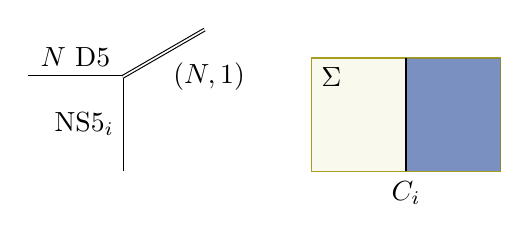
\begin{tikzpicture}[scale=1.2] %, baseline=(x.base)]    \node (x) at (0,0) {\vphantom{x}};

        \draw[xshift=0.01cm] (0,0) -- node[left] {NS5$_i$} ++(0,1);% -- ++(30:1);
        \draw[yshift=0.01cm] (-1,1) -- node[above] {$N$ D5} ++(1,0);% -- ++(30:1);
        \draw[double] (0,1) -- node[below right] {$(N,1)$} ++(30:1);

        \filldraw[color=olive!80, fill=olive!5] (2,1.2) node[color=black, below right] {$\Sigma$} rectangle (4,0);
        \filldraw[color=olive!80, fill=cyan!20!blue, opacity=0.6] (3,0) rectangle (4,1.2);
        \draw[semithick] (3,0) node[below] {$C_i$} -- ++(0,1.2);

    \end{tikzpicture}
    }
  \qquad\qquad
  \subfloat[\label{fig:(N,-1)}]{

    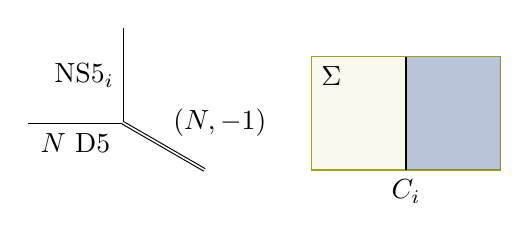
\begin{tikzpicture}[scale=1.2] %, baseline=(x.base)]    \node (x) at (0,0) {\vphantom{x}};
        \def\shift{0.5cm}
        \draw[xshift=0.01cm, yshift=\shift] (0,0) -- node[left] {NS5$_i$} ++(0,1);% -- ++(30:1);
        \draw[yshift=-0.01cm+\shift] (-1,0) -- node[below] {$N$ D5} ++(1,0);% -- ++(30:1);
        \draw[double,yshift=\shift] (0,0) -- node[above right] {$(N,-1)$} ++(-30:1);

        \filldraw[color=olive!80, fill=olive!5] (2,1.2) node[color=black, below right] {$\Sigma$} rectangle (4,0);
        \filldraw[color=olive!80, fill=cyan!20!blue, opacity=0.3] (3,0) rectangle (4,1.2);
        \draw[semithick] (3,0) node[below] {$C_i$} -- ++(0,1.2);

    \end{tikzpicture}
    }
  \caption{An NS5-brane combines with a stack of $N$ D5-branes, forming (a) and $(N,1)$ 5-brane
  or (b) an $(N,-1)$ 5-brane. The 5-brane junction is a domain wall in $\mathsf{T}_{\mathrm{D5}}$.
  The shaded regions shown above support a nonzero NS5-brane charge $q=\pm 1$}
  \label{fig:D5NS5config}
\end{figure}


Conversely, given a configuration of curves $C_{i}$ on the two-dimensional
surface $\Sigma$ and a 5-brane charge assignment consistent with
it, we can construct a 5-brane system whose zig-zag paths are $C_{i}$:
we take NS5-branes approaching the D5-branes from transverse directions,
and let them meet along $C_{i}$ and form bound states over regions
with $q \neq 0$. Such a 5-brane system is called a brane tiling on
$\Sigma$ \cite{Hanany:2005ve,Franco:2005rj}.

As we just explained, a brane tiling gives rise to a four-dimensional
$\mathcal{N}=1$ theory. A concrete description of this theory is
known for the subset of brane tilings that involve only $\left( N,0 \right)$
5-branes (i.e. $N$ coincident D5-branes) and $\left( N,\pm1 \right)$
5-branes. Given a brane tiling in this subset, we indicate $\left( N,1 \right)$
and $\left( N,-1 \right)$ 5-brane regions by dark and light shading,
respectively, while leaving $\left( N,0 \right)$ regions unshaded.
After the shading, we get a checkerboard-like pattern on $\Sigma$
where shaded faces adjoin unshaded ones and two shaded faces sharing
a vertex are of different types, see figure.


%FIGURE    to be fixed
\begin{figure}
\centering
\def\width{3cm}
\def\height{2cm}
  \subfloat[\label{}]{
    \begin{tikzpicture}[scale=1] %, baseline=(x.base)]    \node (x) at (0,0) {\vphantom{x}};
        \def\step{0.15cm}
        \def\shift{0.25cm}
        \def\sep{1cm}

        \fill[fill=olive!5] (0,0) rectangle (\width,\height);

        \fill[lightshade] (0,0) rectangle (\step,\step);
        \fill[lightshade] (\step+\shift,0) rectangle (\step+\sep,\step);    % ????
        \fill[lightshade] (\step+\shift+\sep,0) rectangle (\step+2*\sep,\step);    % ????
        \fill[lightshade] (\step+\shift+2*\sep,0) rectangle (\width,\step);    % ????

        \fill[lightshade] (0,\step+\shift) rectangle (\step,\step+\sep);
        \fill[lightshade] (\step+\shift,\step+\shift) rectangle (\step+\sep,\step+\sep);
        \fill[lightshade] (\step+\shift+\sep,\step+\shift) rectangle (\step+2*\sep,\step+\sep);
        \fill[lightshade] (\step+\shift+2*\sep,\step+\shift) rectangle (\width,\step+\sep);

        \fill[lightshade] (0,\step+\shift+\sep) rectangle (\step,\height);
        \fill[lightshade] (\step+\shift,\step+\shift+\sep) rectangle (\step+\sep,\height);
        \fill[lightshade] (\step+\shift+\sep,\step+\shift+\sep) rectangle (\step+2*\sep,\height);
        \fill[lightshade] (\step+\shift+2*\sep,\step+\shift+\sep) rectangle (\width,\height);

        \fill[darkshade] (\step,\step) rectangle (\step+\shift,\step+\shift);
        \fill[darkshade, xshift=\sep] (\step,\step) rectangle (\step+\shift,\step+\shift);
        \fill[darkshade, xshift=2*\sep] (\step,\step) rectangle (\step+\shift,\step+\shift);

        \begin{scope}[yshift=\sep]
        \fill[darkshade] (\step,\step) rectangle (\step+\shift,\step+\shift);
        \fill[darkshade, xshift=\sep] (\step,\step) rectangle (\step+\shift,\step+\shift);
        \fill[darkshade, xshift=2*\sep] (\step,\step) rectangle (\step+\shift,\step+\shift);
        \end{scope}

        \draw[semithick] (\step,0) -- ++(0,\height);
        \draw[semithick, xshift=\shift] (\step,0) -- ++(0,\height);
        \draw[semithick, xshift=\sep] (\step,0) -- ++(0,\height);
        \draw[semithick, xshift=\sep+\shift] (\step,0) -- ++(0,\height);
        \draw[semithick, xshift=2*\sep] (\step,0) -- ++(0,\height);
        \draw[semithick, xshift=2*\sep+\shift] (\step,0) -- ++(0,\height);

        \draw[semithick] (0,\step) -- ++(\width,0);
        \draw[semithick, yshift=\shift] (0,\step) -- ++(\width,0);
        \draw[semithick, yshift=\sep] (0,\step) -- ++(\width,0);
        \draw[semithick, yshift=\sep+\shift] (0,\step) -- ++(\width,0);

        \draw[color=olive!80] (0,0) rectangle (\width,\height);


    \end{tikzpicture}
    }
  \quad
  \subfloat[\label{}]{
    \begin{tikzpicture}[scale=1] %, baseline=(x.base)]    \node (x) at (0,0) {\vphantom{x}};
        \useasboundingbox (0,0) rectangle (\width,\height);

        \def\step{0.15cm}
        \def\shift{0.25cm}
        \def\sep{1cm}
        \def\site{\shift+\sep/2}

        \node[node, minimum size=7pt] (a1) at (\site,\step+\shift/2) {};  %%%%
        \node[node, minimum size=7pt, xshift=\sep] (a2) at (\site,\step+\shift/2) {};
        \node[node, minimum size=7pt, xshift=2*\sep] (a3) at (\site,\step+\shift/2) {};
        \node[node, minimum size=7pt] (b1) at (\step+\shift/2,\site) {};  %%%%
        \node[node, minimum size=7pt, xshift=\sep] (b2) at (\step+\shift/2,\site) {};
        \node[node, minimum size=7pt, xshift=2*\sep] (b3) at (\step+\shift/2,\site) {};
        \begin{scope}[yshift=\sep]
        \node[node, minimum size=7pt] (c1) at (\site,\step+\shift/2) {};  %%%%
        \node[node, minimum size=7pt, xshift=\sep] (c2) at (\site,\step+\shift/2) {};
        \node[node, minimum size=7pt, xshift=2*\sep] (c3) at (\site,\step+\shift/2) {};
        \node[node, minimum size=7pt] (d1) at (\step+\shift/2,\site) {};  %%%%
        \node[node, minimum size=7pt, xshift=\sep] (d2) at (\step+\shift/2,\site) {};
        \node[node, minimum size=7pt, xshift=2*\sep] (d3) at (\step+\shift/2,\site) {};
        \end{scope}

        \draw[semithick, arrows=-latex] (b1) to (a1); \draw[semithick, arrows=-latex] (a1) to (b2); \draw[semithick, arrows=-latex] (b2) to (a2); \draw[semithick, arrows=-latex] (a2) to (b3); \draw[semithick, arrows=-latex] (b3) to (a3);
        \draw[semithick, arrows=-latex] (c1) to (b1); \draw[semithick, arrows=-latex] (b2) to (c1); \draw[semithick, arrows=-latex] (c2) to (b2); \draw[semithick, arrows=-latex] (b3) to (c2); \draw[semithick, arrows=-latex] (c3) to (b3);
        \draw[semithick, arrows=-latex] (d1) to (c1); \draw[semithick, arrows=-latex] (c1) to (d2); \draw[semithick, arrows=-latex] (d2) to (c2); \draw[semithick, arrows=-latex] (c2) to (d3); \draw[semithick, arrows=-latex] (d3) to (c3);

        \path[name path=rec, draw=none] (0,0) rectangle (\width,\height);
        \path[name path=quiv1, draw=none] (a1) to (\step+\shift/2,\site-\sep);
        \path[name path=quiv2, draw=none] (a1) to (\step+\shift/2+\sep,\site-\sep);
        \path[name intersections={of= rec and quiv1, by={A}}];\tikzmath{coordinate \a;  \a = (A);}    % actually \ay=0!!
        \path[name intersections={of= rec and quiv2, by={B}}];\tikzmath{coordinate \b;  \b = (B);}    % actually \by=0!!

        \draw[semithick] (\ax,0) to (a1); \draw[semithick, arrows=-latex] (\bx,0) to (a1);
        \draw[semithick] (\ax+\sep,0) to (a2); \draw[semithick, arrows=-latex] (\bx+\sep,0) to (a2);
        \draw[semithick] (\ax+2*\sep,0) to (a3); \draw[semithick, arrows=-latex] (\width,0) to (a3);  %\bx+2*\sep

        \draw[semithick, arrows=-latex] (0,\ax) to (b1); \draw[semithick] (0,\bx) to (b1);
        \draw[semithick, arrows=-latex] (0,\ax+\sep) to (d1);

        \draw[semithick] (\width-\bx,\height) to (d3); \draw[semithick, arrows=-latex] (\width-\ax,\height) to (d3);
        \draw[semithick] (\width-\bx-\sep,\height) to (d2); \draw[semithick, arrows=-latex] (\width-\ax-\sep,\height) to (d2);
        \draw[semithick] (0,\height) to (d1); \draw[semithick, arrows=-latex] (\width-\ax-2*\sep,\height) to (d1);

        \draw[semithick] (\width,\height-\ax) to (c3); \draw[semithick, arrows=-latex] (\width,\height-\bx) to (c3);
        \draw[semithick] (\width,\height-\ax-\sep) to (a3);

        \draw[color=olive!80] (0,0) rectangle (\width,\height);

    \end{tikzpicture}
    }
  \quad
  \subfloat[\label{}]{
      \begin{tikzpicture}[scale=1] %, baseline=(x.base)]    \node (x) at (0,0) {\vphantom{x}};
        \def\step{0.15cm}
        \def\shift{0.25cm}
        \def\sep{1cm}

        \path[name path=v1, draw=none] (\step+\sep/2,0) -- ++(0,\height);
        \path[name path=l1, draw=none] (\step+\sep/2-\shift,0) -- ++(\height,\height);    % canonical line
        \path[name intersections={of= v1 and l1, by={A}}];\tikzmath{coordinate \ca;  \ca = (A);}

        \fill[fill=olive!5] (0,0) rectangle (\width,\height);

        \fill[darkshade] (\step+\sep/2-\shift,0) -- (\step+\sep/2,0) -- (\cax,\cay) -- cycle;
        \fill[lightshade] (\step+\sep/2,\step+\sep/2) -- (\cax,\cay) -- (\step+\sep/2-\shift+\cax,\step+\sep/2) -- cycle;
        \fill[darkshade] (\step+\sep/2,\step+\sep/2) -- (\cax,\cay+\sep) -- (0,\step+\sep/2) -- cycle;
        \fill[lightshade, yshift=\sep] (\step+\sep/2,\step+\sep/2) -- (\cax,\cay) -- (\step+\sep/2-\shift+\cax,\step+\sep/2) -- cycle;
        \fill[darkshade] (0,\step+\sep/2+\sep) -- (\step+\sep/2,\step+\sep/2+\sep) -- (\step+\sep/2,\height) -- (\step+\sep/2-\shift,\height) -- cycle;

        \begin{scope}[xshift=\sep]
        \fill[darkshade] (\step+\sep/2-\shift,0) -- (\step+\sep/2,0) -- (\cax,\cay) -- cycle;
        \fill[lightshade] (\step+\sep/2,\step+\sep/2) -- (\cax,\cay) -- (\step+\sep/2-\shift+\cax,\step+\sep/2) -- cycle;
        \fill[darkshade] (\step+\sep/2,\step+\sep/2) -- (\cax,\cay+\sep) -- (0,\step+\sep/2) -- cycle;
        \fill[lightshade, yshift=\sep] (\step+\sep/2,\step+\sep/2) -- (\cax,\cay) -- (\step+\sep/2-\shift+\cax,\step+\sep/2) -- cycle;
        \fill[darkshade] (0,\step+\sep/2+\sep) -- (\step+\sep/2,\step+\sep/2+\sep) -- (\step+\sep/2,\height) -- (\step+\sep/2-\shift,\height) -- cycle;
        \end{scope}

        \begin{scope}[xshift=2*\sep]
        \fill[darkshade] (\step+\sep/2-\shift,0) -- (\step+\sep/2,0) -- (\cax,\cay) -- cycle;
        \fill[lightshade] (\step+\sep/2,\step+\sep/2) -- (\cax,\cay) -- (\step+\sep/2-\shift+\cax,\step+\sep/2) -- cycle;
        \fill[darkshade] (\step+\sep/2,\step+\sep/2) -- (\cax,\cay+\sep) -- (0,\step+\sep/2) -- cycle;
        \fill[lightshade, yshift=\sep] (\step+\sep/2,\step+\sep/2) -- (\cax,\cay) -- (\step+\sep/2-\shift+\cax,\step+\sep/2) -- cycle;
        \fill[darkshade] (0,\step+\sep/2+\sep) -- (\step+\sep/2,\step+\sep/2+\sep) -- (\step+\sep/2,\height) -- (\step+\sep/2-\shift,\height) -- cycle;
        \end{scope}

        % vertical lines
        \draw[semithick] (\step+\sep/2,0) -- ++(0,\height);
        \draw[semithick, xshift=\sep] (\step+\sep/2,0) -- ++(0,\height);
        \draw[semithick, xshift=2*\sep] (\step+\sep/2,0) -- ++(0,\height);

        % horizontal lines
        \draw[semithick] (0,\step+\sep/2) -- ++(\width,0);
        \draw[semithick, yshift=\sep] (0,\step+\sep/2) -- ++(\width,0);

        \draw[semithick] (0,\step+\sep/2+\sep) -- (\step+\sep/2-\shift,\height);
        \draw[semithick] (0,\step+\sep/2) -- (\step+\sep/2+\sep-\shift,\height);
        \draw[semithick] (\step+\sep/2-\shift,0) -- ++(\height,\height);    % canonical line
        \draw[semithick] (\step+\sep/2-\shift+\sep,0) -- (\width,\step+\sep/2+\sep);
        \draw[semithick] (\step+\sep/2-\shift+2*\sep,0) -- (\width,\step+\sep/2);

        \draw[color=olive!80] (0,0) rectangle (\width,\height);

    \end{tikzpicture}
  }
  \quad
  \subfloat[\label{}]{
    \begin{tikzpicture}[scale=1] %, baseline=(x.base)]    \node (x) at (0,0) {\vphantom{x}};
        \useasboundingbox (0,0) rectangle (\width,\height);

        \def\step{0.15cm}
        \def\shift{0.25cm}
        \def\sep{1cm}
        \def\site{2*\step}

        \node[fnode, minimum size=7pt] (a1) at (1.2*\site,\site) {};
        \node[fnode, minimum size=7pt, xshift=\sep] (a2) at (1.2*\site,\site) {};
        \node[fnode, minimum size=7pt, xshift=2*\sep] (a3) at (1.2*\site,\site) {};

        \begin{scope}[yshift=0.7*\sep]
        \node[node, minimum size=7pt] (b1) at (1.2*\site,\site) {};
        \node[node, minimum size=7pt, xshift=\sep] (b2) at (1.2*\site,\site) {};
        \node[node, minimum size=7pt, xshift=2*\sep] (b3) at (1.2*\site,\site) {};
        \end{scope}

        \begin{scope}[yshift=1.4*\sep]
        \node[fnode, minimum size=7pt] (c1) at (1.2*\site,\site) {};
        \node[fnode, minimum size=7pt, xshift=\sep] (c2) at (1.2*\site,\site) {};
        \node[fnode, minimum size=7pt, xshift=2*\sep] (c3) at (1.2*\site,\site) {};
        \end{scope}

        \draw[semithick, -latex] (a1) to (a2); \draw[semithick, -latex] (a2) to (a3);
        \draw[semithick, -latex] (a1) to (b1); \draw[semithick, -latex] (a2) to (b2); \draw[semithick, -latex] (a3) to (b3);
        \draw[semithick, -latex] (b1) to (b2); \draw[semithick, -latex] (b2) to (b3);
        \draw[semithick, -latex] (b1) to (c1); \draw[semithick, -latex] (b2) to (c2); \draw[semithick, -latex] (b3) to (c3);
        \draw[semithick, -latex] (b2) to (a1); \draw[semithick, -latex] (b3) to (a2);
        \draw[semithick, -latex] (c2) to (b1); \draw[semithick, -latex] (c3) to (b2);


        \path[name path=rec, draw=none] (0,0) rectangle (\width,\height);
        \path[name path=quiv, draw=none] (b1) to (\site-\sep,\site);
        \path[name intersections={of= rec and quiv, by={A}}];\tikzmath{coordinate \ca;  \ca = (A);}    % actually \cax=0!!

        \draw[semithick] (b1) to (\cax,\cay); \draw[semithick] (c1) to (\cax,\cay+0.7*\sep);
        \draw[semithick, -latex] (0,\site) to (a1); \draw[semithick, -latex] (0,\site+0.7*\sep) to (b1);

        \draw[semithick, -latex] (\width,\cay) to (a3); \draw[semithick, -latex] (\width,\cay+0.7*\sep) to (b3);
        \draw[semithick] (a3) to (\width,\site); \draw[semithick] (b3) to (\width,\site+0.7*\sep);

        \draw[color=olive!80] (0,0) rectangle (\width,\height);

    \end{tikzpicture}
    }
  \caption{(a) A brane tiling on a torus. (b) The periodic quiver associated with (a).
  (c) A brane tiling on a finite-length cylinder. (d) the quiver for (c).}
  \label{fig:tilings_quiverdiagram}
\end{figure}


Each unshaded region supports $N$ D5-branes, hence an $\SU(N)$ vector
multiplet lives there. If the region contains part of the boundary,
the multiplet is frozen by boundary conditions and the associated
symmetry is an $\SU(N)$ flavor symmetry; in quiver notation, we represent
a dynamical vector multiplet by a gauge node (circle) and a non-dynamical
one by a flavor node (square). From open strings stretched between
two unshaded regions (namely ending on $N$ D5-branes partitioned
by NS5-brane) sharing a vertex, we get a chiral multiplet that transforms
in the fundamental representation under one of the associated gauge
or flavor groups and in the anti-fundamental representation under
the other. We write it by an arrow between the two nodes:
\begin{equation}
    \begin{tikzpicture}[scale=1.2, baseline=(x.base)]    \node (x) at (0,0) {\vphantom{x}};

        \fill[color=olive!5] (-0.5,-0.5) rectangle (0.5,0.5);
        \fill[darkshade] (0.5,-0.5) -- (0.5,0.5) -- (0,0) -- cycle;
        \fill[lightshade] (-0.5,0.5) -- (-0.5,-0.5) -- (0,0) -- cycle;

        \draw (-0.5,-0.5) node[below] {$i$} -- ++(45:{sqrt(2)});
        \draw (0.5,-0.5) node[below] {$j$} -- ++(135:{sqrt(2)});

    \end{tikzpicture}
  %
  \quad  \rightsquigarrow  \quad
  %
    \begin{tikzpicture}[scale=1, baseline=(x.base)]    \node (x) at (0,0) {\vphantom{x}};

        \node[fnode] (a) at (0,-0.5) {};
        \node[fnode] (b) at (0,0.5) {};
        \draw[semithick, arrows=-latex] (a) to (b);

    \end{tikzpicture}
  \quad .
  \label{eq:bifund}
\end{equation}
 The arrow points from the anti-fundamental side to the fundamental
side. See figure \ref{fig:tilings_quiverdiagram} for examples of quivers obtained from brane tilings.

Moreover, for every set of zig-zag paths bounding a shaded region,
we have a loop of arrows and world-sheet instantons generate a superpotential
term given by the trace of the product of the bifundamental chiral
multiplets in the loop. The coefficient of this term is positive or
negative depending on whether the direction of the loop is clockwise
or counterclockwise. Thus, the four-dimensional theory realized by
a brane tiling in the subset under consideration is an $\mathcal{N}=1$
supersymmetric gauge theory described by a quiver with potential drawn
on $\Sigma$.

Each NS5$_{i}$ supports a $\U(1)$ flavor symmetry $\U(1)_{i}$. An
arrow is charged under $\U(1)_{i}$ if it is crossed by $C_{i}$. The
charge $F_{i}$ of $\U(1)_{i}$ can be normalized in such a way that
the arrow in (\ref{eq:bifund}) has $F_{i}=-1$ and $F_{j}=+1$. The
diagonal combination of all $\U(1)_{i}$ acts on the theory trivially
since every arrow is crossed by exactly two zig-zag paths from the
opposite sides.

The theory also has an R-symmetry $\U(1)_{R}$. Its definition is not
unique as the R-charge $R$ can be shifted by a linear combination
of $\U(1$) flavor charges. However, the R-charge assignment is constrained
by two conditions. The first is that $\U(1)_{R}$ must be unbroken
by the superpotential and therefore the R-charges of the chiral multiplets
contained in each superpotential term must add up to two. The second
is that $\U(1)_{R}$ must be free of anomaly. This requires that for
every gauge node, the sum of the R-charges of the arrows starting
from or ending at that node must equal the number of the arrows minus
two.

To fix the R-charge assignment, let us assume that we can orient the
zig-zag paths and bound every shaded or unshaded region with zig-zag
paths all heading upward, for some choice of the ``vertical'' direction
in the neighborhood of that region. This is the case for the examples
in figure \ref{fig:tilings_quiverdiagram}. The zig-zag paths thus oriented fall into two groups; when
a zig-zag path goes upward and we cross it from the left to the right,
$q$ increases by one. We distinguish the latter case from the former
by drawing the zig-zag path with a dotted line. Then, we give an arrow
$R=0$ if it originates from a crossing of two zig-zag paths of the
same type, and $R=1$ otherwise. With this R-charge assignment the
two conditions describe above are satisfied (see figure \ref{fig:twoexamples}).


%FIGURE
\begin{figure}
\centering
  \subfloat[\label{}]{
    \begin{tikzpicture}[scale=1] %, baseline=(x.base)]    \node (x) at (0,0) {\vphantom{x}};
        \def\radius{1.2cm}

        \path[name path=dot1, draw=none] (280:\radius) to[bend left=10] (190:\radius);
        \path[name path=dot2, draw=none] (225:\radius) to[bend right=10] (135:\radius);
        \path[name path=dot3, draw=none] (170:\radius) to[bend left=10] (60:\radius);
        \path[name path=solid1, draw=none] (260:\radius) to[bend left=10] (340:\radius);
        \path[name path=solid2, draw=none] (315:\radius) to[bend left=10] (30:\radius);
        \path[name path=solid3, draw=none] (0:\radius) -- (100:\radius);

        \path[name intersections={of= dot1 and solid1, by={A}}];
        \path[name intersections={of= dot1 and dot2, by={B}}];
        \path[name intersections={of= dot2 and dot3, by={C}}];
        \path[name intersections={of= dot3 and solid3, by={D}}];
        \path[name intersections={of= solid2 and solid3, by={E}}];
        \path[name intersections={of= solid1 and solid2, by={F}}];

        \fill[olive!5] (0,0) circle[radius=\radius];

        \fill[darkshade] (A) to (260:\radius) arc (260:280:\radius) -- cycle;
        \fill[darkshade] (B) to (190:\radius) arc (190:225:\radius) -- cycle;
        \fill[darkshade] (C) to (135:\radius) arc (135:170:\radius) -- cycle;
        \fill[darkshade] (D) to (60:\radius) arc (60:100:\radius) -- cycle;
        \fill[darkshade] (E) to (0:\radius) arc (0:30:\radius) -- cycle;
        \fill[darkshade] (F) to (315:\radius) arc (315:340:\radius) -- cycle;

        \fill[lightshade] (A) to[bend left=5] (B) to[bend right=5] (C) to[bend left=5] (D) -- (E) to[bend right=5] (F) to[bend right=5] cycle;

        \draw[semithick, densely dotted, ->] (280:\radius) to[bend left=10] (190:\radius);
        \draw[semithick, densely dotted, ->] (225:\radius) to[bend right=10] (135:\radius);
        \draw[semithick, densely dotted, ->] (170:\radius) to[bend left=10] (60:\radius);
        \draw[semithick, ->] (260:\radius) to[bend left=10] (340:\radius);
        \draw[semithick, ->] (315:\radius) to[bend left=10] (30:\radius);
        \draw[semithick, ->] (0:\radius) -- (100:\radius);

        \begin{scope}[scale=0.8]
        \node[fnode, xshift=2.4*\radius] (a) at (350:\radius) {};\node[fnode, xshift=2.4*\radius] (b) at (45:\radius) {};
        \node[fnode, xshift=2.4*\radius] (c) at (235/2:\radius) {};\node[fnode, xshift=2.4*\radius] (d) at (180:\radius) {};
        \node[fnode, xshift=2.4*\radius] (e) at (485/2:\radius) {};\node[fnode, xshift=2.4*\radius] (f) at (595/2:\radius) {};
        \draw[semithick, arrows=-latex] (a) -- (b);\draw[semithick, arrows=-latex] (b) -- (c);\draw[semithick, arrows=-latex] (c) -- (d);
        \draw[semithick, arrows=-latex] (d) -- (e);\draw[semithick, arrows=-latex] (e) -- (f);\draw[semithick, arrows=-latex] (f) -- (a);
        \end{scope}

    \end{tikzpicture}
    }
  %
  \qquad\qquad
  %
  \subfloat[\label{}]{
    \begin{tikzpicture}[scale=1] %, baseline=(x.base)]    \node (x) at (0,0) {\vphantom{x}};
        \def\radius{1.2cm}

        \path[name path=dot1, draw=none] (280:\radius) to[bend left=10] (190:\radius);
        \path[name path=dot2, draw=none] (225:\radius) to[bend right=10] (135:\radius);
        \path[name path=dot3, draw=none] (170:\radius) to[bend left=10] (60:\radius);
        \path[name path=solid1, draw=none] (260:\radius) to[bend left=10] (340:\radius);
        \path[name path=solid2, draw=none] (315:\radius) to[bend left=10] (30:\radius);
        \path[name path=solid3, draw=none] (0:\radius) -- (100:\radius);

        \path[name intersections={of= dot1 and solid1, by={A}}];
        \path[name intersections={of= dot1 and dot2, by={B}}];
        \path[name intersections={of= dot2 and dot3, by={C}}];
        \path[name intersections={of= dot3 and solid3, by={D}}];
        \path[name intersections={of= solid2 and solid3, by={E}}];
        \path[name intersections={of= solid1 and solid2, by={F}}];

        \fill[olive!5] (0,0) circle[radius=\radius];

        \fill[darkshade] (A) to[bend left=5] (B) to (225:\radius) arc (225:260:\radius) --(A) -- cycle;
        \fill[lightshade] (B) to[bend right=5] (C) to (170:\radius) arc (170:190:\radius) -- (B) -- cycle;
        \fill[darkshade] (C) to[bend left=5] (D) to (100:\radius) arc (100:135:\radius) -- (C) -- cycle;
        \fill[lightshade] (D) to (E) to (30:\radius) arc (30:60:\radius) -- (D) -- cycle;
        \fill[darkshade] (E) to[bend right=5] (F) to (340:\radius) arc (340:360:\radius) -- (E) -- cycle;
        \fill[lightshade] (F) to[bend right=5] (A) to (280:\radius) arc (280:315:\radius) (F) -- cycle;

        %\fill[lightshade] (A) to[bend left=5] (B) to[bend right=5] (C) to[bend left=5] (D) -- (E) to[bend right=5] (F) to[bend right=5] cycle;

        \draw[semithick, densely dotted, ->] (280:\radius) to[bend left=10] (190:\radius);
        \draw[semithick, ->] (225:\radius) to[bend right=10] (135:\radius);
        \draw[semithick, densely dotted, ->] (170:\radius) to[bend left=10] (60:\radius);
        \draw[semithick, densely dotted, ->] (260:\radius) to[bend left=10] (340:\radius);
        \draw[semithick, ->] (315:\radius) to[bend left=10] (30:\radius);
        \draw[semithick, densely dotted, ->] (0:\radius) -- (100:\radius);

        \begin{scope}[scale=0.8]
        \node[fnode, xshift=2.4*\radius] (a) at (15:\radius) {};\node[fnode, xshift=2.4*\radius] (b) at (80:\radius) {};
        \node[fnode, xshift=2.4*\radius] (c) at (305/2:\radius) {};\node[fnode, xshift=2.4*\radius] (d) at (415/2:\radius) {};
        \node[fnode, xshift=2.4*\radius] (e) at (270:\radius) {};\node[fnode, xshift=2.4*\radius] (f) at (655/2:\radius) {};
        \node[node,  xshift=2.4*\radius] (g) at (0,0) {};
        \draw[semithick, arrows=-latex] (g) -- (a);\draw[semithick, arrows=-latex] (b) -- (g);\draw[semithick, arrows=-latex] (g) -- (c);
        \draw[semithick, arrows=-latex] (d) -- (g);\draw[semithick, arrows=-latex] (g) -- (e);\draw[semithick, arrows=-latex] (f) -- (g);
        \end{scope}

    \end{tikzpicture}
    }
  \caption{Zig-zag paths bounding (a) a shaded region and (b) an unshaded region.
  In either case, the R-charges of two of the arrows are different from those of the rest.}
  \label{fig:twoexamples}
\end{figure}


Summarizing the rules for assignment of the charges, we can read off
the quiver diagram from zig-zag paths as in figure \ref{fig:rule_for_quiver}.

%FIGURE
\begin{figure}
\centering
\newcommand{\shift}{1.3cm}
  \subfloat[\label{}]{
        \begin{tikzpicture}[scale=1.2, baseline=(x.base)]    \node (x) at (0,0) {\vphantom{x}};
        \fill[color=olive!5] (-0.5,-0.5) rectangle (0.5,0.5);
        \fill[darkshade] (0.5,-0.5) -- (0.5,0.5) -- (0,0) -- cycle;
        \fill[lightshade] (-0.5,0.5) -- (-0.5,-0.5) -- (0,0) -- cycle;

        \draw[semithick, ->] (-0.5,-0.5) node[below] {$i$} -- ++(45:{sqrt(2)});
        \draw[semithick, ->] (0.5,-0.5) node[below] {$j$} -- ++(135:{sqrt(2)});

        \begin{scope}[scale=5/6]
        \node[fnode, xshift=\shift] (a) at (0,-0.5) {};
        \node[fnode, xshift=\shift] (b) at (0,0.5) {};
        \draw[semithick, arrows=-latex, xshift=\shift] (a) to (b);
        \end{scope}
    \end{tikzpicture}
    }
  \qquad
  \subfloat[\label{}]{
        \begin{tikzpicture}[scale=1.2, baseline=(x.base)]    \node (x) at (0,0) {\vphantom{x}};
        \fill[color=olive!5] (-0.5,-0.5) rectangle (0.5,0.5);
        \fill[lightshade] (0.5,-0.5) -- (0.5,0.5) -- (0,0) -- cycle;
        \fill[darkshade] (-0.5,0.5) -- (-0.5,-0.5) -- (0,0) -- cycle;

        \draw[semithick, densely dotted, ->] (-0.5,-0.5) node[below] {$i$} -- ++(45:{sqrt(2)});
        \draw[semithick, densely dotted, ->] (0.5,-0.5) node[below] {$j$} -- ++(135:{sqrt(2)});

        \begin{scope}[scale=5/6]
        \node[fnode, xshift=\shift] (a) at (0,-0.5) {};
        \node[fnode, xshift=\shift] (b) at (0,0.5) {};
        \draw[semithick, arrows=-latex, xshift=\shift] (b) to (a);
        \end{scope}
    \end{tikzpicture}
    }
  \qquad
  \subfloat[\label{}]{
        \begin{tikzpicture}[scale=1.2, baseline=(x.base)]    \node (x) at (0,0) {\vphantom{x}};
        \fill[color=olive!5] (-0.5,-0.5) rectangle (0.5,0.5);
        \fill[darkshade] (-0.5,-0.5) -- (0.5,-0.5) -- (0,0) -- cycle;
        \fill[lightshade] (0.5,0.5) -- (-0.5,0.5) -- (0,0) -- cycle;

        \draw[semithick, ->] (-0.5,-0.5) node[below] {$i$} -- ++(45:{sqrt(2)});
        \draw[semithick, densely dotted, ->] (0.5,-0.5) node[below] {$j$} -- ++(135:{sqrt(2)});

        \begin{scope}[scale=5/6]
        \node[fnode, xshift=\shift] (a) at (0,0) {};
        \node[fnode, xshift=\shift] (b) at (1,0) {};
        \draw[semithick, arrows=-latex, xshift=\shift] (a) to (b);
        \end{scope}
    \end{tikzpicture}
    }
  \qquad
  \subfloat[\label{}]{
        \begin{tikzpicture}[scale=1.2, baseline=(x.base)]    \node (x) at (0,0) {\vphantom{x}};
        \fill[color=olive!5] (-0.5,-0.5) rectangle (0.5,0.5);
        \fill[darkshade] (0.5,0.5) -- (-0.5,0.5) -- (0,0) -- cycle;
        \fill[lightshade] (-0.5,-0.5) -- (0.5,-0.5) -- (0,0) -- cycle;

        \draw[semithick, densely dotted, ->] (-0.5,-0.5) node[below] {$i$} -- ++(45:{sqrt(2)});
        \draw[semithick, ->] (0.5,-0.5) node[below] {$j$} -- ++(135:{sqrt(2)});

        \begin{scope}[scale=5/6]
        \node[fnode, xshift=\shift] (a) at (0,0) {};
        \node[fnode, xshift=\shift] (b) at (1,0) {};
        \draw[semithick, arrows=-latex, xshift=\shift] (b) to (a);
        \end{scope}
    \end{tikzpicture}
    }
  \caption{The rule for assigning a quiver to a brane tiling diagram.
  The arrows in (a) and (b) have $(R, F_i, F_j)=(0, -1, 1)$. Those in
  (c) and (d) have $(R, F_i, F_j)=(1, 1, -1)$.}
  \label{fig:rule_for_quiver}
\end{figure}





\subsubsection{Integrable lattice models from quiver gauge theories}

From the supersymmetric index of the four-dimensional $\mathcal{N}=1$
theory realized by a brane tiling, we obtain an integrable lattice
model defined on the lattice $\left\{ C_{i}\right\} $ consisting
of the zig-zag paths. Each $C_{i}$ carries a spectral parameter $u_{i}$.
S-duality followed by T-duality on $S^{1}$ turns NS5$_{i}$ into
a D4-brane, and its coordinate on the dual circle $\check{S}^{1}$
is $u_{i}$. Instead, we can apply T-duality on $S^{1}$ and lift
NS5$_{i}$ to an M5-brane, then $u_{i}$ is the coordinate on the
M-theory circle. Either way, $u_{i}$ is determined by the holonomy
of the $\U(1)$ gauge field on NS5$_{i}$ along $S^{1}$.

If the theory is described by a quiver, translation between the gauge
theory and the lattice model goes as follows \cite{Yamazaki:2012cp,Yamazaki:2013nra}.
Nodes are interpreted as spin sites. For each flavor node, we can
turn on a holonomy of the associated gauge field. The index depends
on the conjugacy class of the holonomy, which is uniquely represented
by a diagonal matrix $\mathrm{diag}(z_{1},\ldots,z_{N})$ up to permutations
of the entries. The index is therefore a symmetric function of the
$\U(1)$-valued variables $(z_{1},\ldots,z_{N})$ obeying the constraint
$z_{1}\cdots z_{N}=1$. These variables are fugacities for the $\SU(N)$
flavor symmetry and parametrize the value of the spin at this node,
and thus the spins take values in the maximal torus $\U(1)^{N-1}$
of $\SU(N)$. For a gauge node, integration is performed over the fugacities
since its gauge field is a path integral variable. This is the summation
over the values of a spin placed on an internal face. Finally, arrows
represent interactions between spins.

The unitarity relations are satisfied if the contributions to the
index from arrows with $R=0$ are properly normalized. For example,
consider the relation
\begin{equation}
    \begin{tikzpicture}[yscale=0.6, baseline=(x.base)]    \node (x) at (0,0) {\vphantom{x}};

        \path[name path=line1, draw=none] (0,0.4) to[out=0, in=180] (1,-0.4) to[out=0, in=180] (2,0.4);
        \path[name path=line2, draw=none] (0,-0.4) to[out=0, in=180] (1,0.4) to[out=0, in=180] (2,-0.4);
        \path[name intersections={of= line1 and line2, by={A, B}}]; % node at (A) {A} node at (B) {B};

        \fill[olive!5] (0,-0.8) rectangle (2,0.8);

        \fill[lightshade] (0,0.4) to[out=0, in=130] (A) to[out=50, in=180] (1,0.4) to[out=0, in=130] (B) to[out=50, in=180] (2,0.4) -- ++(0,0.4) -- ++(-2,0) -- cycle;
        \fill[darkshade] (0,-0.4) to[out=0, in=230] (A) to[out=310, in=180] (1,-0.4) to[out=0, in=230] (B) to[out=310, in=180] (2,-0.4) -- ++(0,-0.4) -- ++(-2,0) -- cycle;

        \draw[semithick, ->] (0,0.4) to[out=0, in=180] (1,-0.4) to[out=0, in=180] (2,0.4);
        \draw[semithick, ->] (0,-0.4) to[out=0, in=180] (1,0.4) to[out=0, in=180] (2,-0.4);


    \end{tikzpicture}
  \ =
    \begin{tikzpicture}[yscale=0.6, baseline=(x.base)]    \node (x) at (0,0) {\vphantom{x}};

        \fill[olive!5] (0,-0.8) rectangle (2,0.8);

        \fill[lightshade] (0,0.4) -- ++(2,0) -- ++(0,0.4) -- ++(-2,0) -- cycle;
        \fill[darkshade] (0,-0.4) -- ++(2,0) -- ++(0,-0.4) -- ++(-2,0) -- cycle;

        \draw[semithick, ->] (0,0.4) -- (2,0.4);
        \draw[semithick, ->] (0,-0.4) -- (2,-0.4);

    \end{tikzpicture}
  %
  \quad  \Longleftrightarrow  \quad
  %
    \begin{tikzpicture}[scale=1, baseline=(x.base)]    \node (x) at (0,0) {\vphantom{x}};

        \node[fnode] (a) at (-1,0) {};\node[node] (b) at (0,0) {};\node[fnode] (c) at (1,0) {};
        \draw[semithick, arrows=-latex] (a) to (b);\draw[semithick, arrows=-latex] (b) to (c);

    \end{tikzpicture}
  %
  \ = \
  %
    \begin{tikzpicture}[scale=1, baseline=(x.base)]    \node (x) at (0,0) {\vphantom{x}};

        \node[fnode] (a) at (0,0) {};\node[fnode] (b) at (1.2,0) {};
        \draw[eq-] (a) to (b);

    \end{tikzpicture}
\label{eq:unitarity_delta}
\end{equation}
 where the right-hand side is a ``delta function'' that equates
two flavor nodes when one of them is gauged. The precise meaning will
be given for the $S^{1}\times S^{3}$ case below. The theory on the
left-hand side is SQCD with $N$ colors and $N$ flavors. If exhibits
confinement and has a vacuum in which the mesons take nonzero expectation
values and the flavor symmetry $\SU(N)\times \SU(N)$ is broken to the
diagonal subgroup \cite{Seiberg:1994bz}. The index computed in this vacuum
is given by the right-hand side, provided that we cancel the contributions
from the surviving baryon and anti-baryon. Another unitarity relation
\begin{equation}
    \begin{tikzpicture}[yscale=0.6, baseline=(x.base)]    \node (x) at (0,0) {\vphantom{x}};

        \path[name path=line1, draw=none] (0,0.4) to[out=0, in=180] (1,-0.4) to[out=0, in=180] (2,0.4);
        \path[name path=line2, draw=none] (0,-0.4) to[out=0, in=180] (1,0.4) to[out=0, in=180] (2,-0.4);
        \path[name intersections={of= line1 and line2, by={A, B}}]; % node at (A) {A} node at (B) {B};

        \fill[olive!5] (0,-0.8) rectangle (2,0.8);

        \fill[lightshade] (A) to[out=50, in=180] (1,0.4) to[out=0, in=130] (B) to[out=230, in=0] (1,-0.4) to[out=180, in=310]  (A) -- cycle;
        \fill[darkshade] (0,-0.4) to[out=0, in=230] (A) to[out=130, in=0] (0,0.4) -- cycle;
        \fill[darkshade] (2,-0.4) to[out=180, in=310] (B) to[out=50, in=180] (2,0.4) -- cycle;

        \draw[semithick, ->] (0,0.4) to[out=0, in=180] (1,-0.4) to[out=0, in=180] (2,0.4);
        \draw[semithick, densely dotted, ->] (0,-0.4) to[out=0, in=180] (1,0.4) to[out=0, in=180] (2,-0.4);


    \end{tikzpicture}
  \ =
    \begin{tikzpicture}[yscale=0.6, baseline=(x.base)]    \node (x) at (0,0) {\vphantom{x}};

        \fill[olive!5] (0,-0.8) rectangle (2,0.8);

        \fill[darkshade] (0,-0.4) -- ++(2,0) -- ++(0,0.8) -- ++(-2,0) -- cycle;

        \draw[semithick, ->] (0,0.4) -- (2,0.4);
        \draw[semithick, densely dotted, ->] (0,-0.4) -- (2,-0.4);

    \end{tikzpicture}
  %
  \quad  \Longleftrightarrow  \quad
  %
    \begin{tikzpicture}[scale=1, baseline=(x.base)]    \node (x) at (0,0) {\vphantom{x}};

        \node[fnode] (a) at (0,-0.5) {};\node[fnode] (b) at (0,0.5) {};
        \draw[semithick, arrows=-latex] (a) to[bend right=30] (b);\draw[semithick, arrows=-latex] (b) to[bend right=30] (a);

    \end{tikzpicture}
  %
  \ = \
  %
    \begin{tikzpicture}[scale=1, baseline=(x.base)]    \node (x) at (0,0) {\vphantom{x}};

        \node[fnode] (a) at (0,-0.5) {};\node[fnode] (b) at (0,0.5) {};

    \end{tikzpicture}
\end{equation}
 holds since the two arrows on the left-hand side form a loop and
generates a mass term in the superpotential. We can send the mass
to infinity so that these arrows decouple from the theory, and are
left with the right-hand side.

The Yang-Baxter equation with three zig-zag paths is harder to understand,
as it always involves and $\left( N,q \right)$ region with $\left| q \right|>1$
and a quiver description is not available. The problem stems from
the fact that our effects are domain walls across which $q$ changes.
To circumvent the difficulty, we take a pair of zig-zag paths of different
types and think of it as a single line:
\begin{equation}
    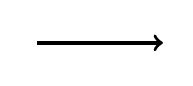
\begin{tikzpicture}[scale=1, baseline=(x.base)]    \node (x) at (0,0) {\vphantom{x}};

        \draw[very thick, ->] (0,0) -- (1.6,0);

    \end{tikzpicture}
  \ = \
    \begin{tikzpicture}[scale=1, baseline=(x.base)]    \node (x) at (0,0) {\vphantom{x}};

        \draw[semithick, ->, yshift=0.2cm] (0,0) -- (1.6,0);
        \draw[semithick, densely dotted, ->, yshift=-0.2cm] (0,0) -- (1.6,0);

    \end{tikzpicture}
\end{equation}
 This line does not alter the value of $q$. Taking two copies of
this line and placing them in an $\left( N,-1 \right)$ background,
we can make the R-matrix
\begin{equation}
    \begin{tikzpicture}[scale=1, baseline=(x.base)]    \node (x) at (0,0) {\vphantom{x}};

        \fill[olive!5] (-1,-1) rectangle (1,1);
        \fill[lightshade] (-1,-1) rectangle (1,1);

        \draw[very thick, ->] (0,-1) -- (0,1);\draw[very thick, ->] (-1,0) -- (1,0);

    \end{tikzpicture}
  %
  \ = \
  %
    \begin{tikzpicture}[scale=1, baseline=(x.base)]    \node (x) at (0,0) {\vphantom{x}};
    \def\shift{0.15cm}

        \fill[olive!5] (-1,-1) rectangle (1,1);
        \fill[lightshade] (\shift,\shift) rectangle (1,1);\fill[lightshade] (-\shift,\shift) rectangle (-1,1);
        \fill[lightshade] (-\shift,-\shift) rectangle (-1,-1);\fill[lightshade] (\shift,-\shift) rectangle (1,-1);
        \fill[darkshade] (-\shift,-\shift) rectangle (\shift,\shift);

        \draw[semithick, ->, xshift=-\shift] (0,-1) -- (0,1);\draw[semithick, ->, yshift=\shift] (-1,0) -- (1,0);
        \draw[semithick, densely dotted, ->, xshift=\shift] (0,-1) -- (0,1);\draw[semithick, densely dotted, ->, yshift=-\shift] (-1,0) -- (1,0);

    \end{tikzpicture}
  %
  \ = \
  %
    \begin{tikzpicture}[scale=0.8, baseline=(x.base)]    \node (x) at (0,0) {\vphantom{x}};

        \node[fnode] (a) at (1,0) {};\node[fnode] (b) at (0,-1) {};\node[fnode] (c) at (-1,0) {};\node[fnode] (d) at (0,1) {};
        \draw[semithick, arrows=-latex] (a) to (b); \draw[semithick, arrows=-latex] (b) to (c);
        \draw[semithick, arrows=-latex] (c) to (d); \draw[semithick, arrows=-latex] (d) to (a);

    \end{tikzpicture}
  \quad .
\label{eq:R_N-1}
\end{equation}
 A lattice model constructed from this R-matrix is a vertex model
whose quiver consists diamonds of arrows (see figure). The vector
space carried by a line is the space of symmetric functions of fugacities
$(z_{1},\ldots,z_{N})$.

Alternatively, we can place these lines in an $\left(N,0\right)$
background and force them to exchange their constituent zig-zag paths
as they cross:
\begin{equation}
    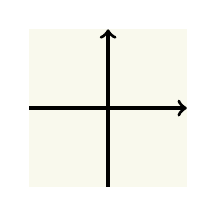
\begin{tikzpicture}[scale=1, baseline=(x.base)]    \node (x) at (0,0) {\vphantom{x}};

        \fill[olive!5] (-1,-1) rectangle (1,1);

        \draw[very thick, ->] (0,-1) -- (0,1);\draw[very thick, ->] (-1,0) -- (1,0);

    \end{tikzpicture}
  %
  \ = \
  %
    \begin{tikzpicture}[scale=1, baseline=(x.base)]    \node (x) at (0,0) {\vphantom{x}};
    \def\shift{0.15}

        \fill[olive!5] (-1,-1) rectangle (1,1);
        \fill[lightshade] (0,0) rectangle (2*\shift,-2*\shift);
        \fill[darkshade] (-1,0) -- (0,0) -- (0,1) -- ++(-2*\shift,0) -- ++(0,2*\shift-1) -- ++(2*\shift-1,0) --cycle;
        \fill[darkshade] (0,-1) -- ++(0,1-2*\shift) -- ++(-2*\shift,0) -- ++(0,2*\shift-1) -- cycle;
        \fill[darkshade] (1,0) -- ++(0,2*\shift) -- ++(2*\shift-1,0) -- ++(0,-2*\shift) -- cycle;

        \draw[semithick, ->] (-2*\shift,-1) -- ++(0,1-2*\shift) -- ++(4*\shift,0) -- ++(0,4*\shift) -- ++(1-2*\shift,0);
        \draw[semithick, ->] (-1,2*\shift) -- ++(1-2*\shift,0) -- ++(0,1-2*\shift);
        \draw[semithick, densely dotted, ->] (0,-1) -- (0,1);
        \draw[semithick, densely dotted, ->] (-1,0) -- (1,0);

    \end{tikzpicture}
  %
  \ = \
  %
    \begin{tikzpicture}[scale=0.6, baseline=(x.base)]    \node (x) at (0,0) {\vphantom{x}};

        \node[fnode] (a) at (1,-1) {};\node[fnode] (b) at (1,1) {};\node[fnode] (c) at (-1,-1) {};
        \draw[semithick, arrows=-latex] (a) to (b);
        \draw[semithick, arrows=-latex] (b) to (c);
        \draw[semithick, arrows=-latex] (c) to (a);

    \end{tikzpicture}
  \quad .
\label{eq:R_N0}
\end{equation}
 This R-matrix leads to an IRF model described by a quiver with triangles
of arrows, as shown in figure. The corresponding Yang-Baxter equation,
after cancellation of some factors with the help of the unitarity
relation (\ref{eq:unitarity_delta}), reads
\begin{equation}
    \begin{tikzpicture}[scale=1.2, baseline=(x.base)]    \node (x) at (0,0) {\vphantom{x}};

        \node[node] (a) at (0,0) {};
        \node[fnode] (b) at (1,0) {};\node[fnode] (c) at (60:1) {};\node[fnode] (d) at (-1,0) {};\node[fnode] (e) at (240:1) {};

        \draw[semithick, ->] (a) to (b);\draw[semithick, ->] (c) to (a);\draw[semithick, ->] (a) to (d);\draw[semithick, ->] (e) to (a);

    \end{tikzpicture}
  %
  \ = \
  %
    \begin{tikzpicture}[scale=1.2, baseline=(x.base)]    \node (x) at (0,0) {\vphantom{x}};

        \node[node] (a) at (0,0) {};
        \node[fnode] (b) at (1,0) {};\node[fnode] (c) at (60:1) {};\node[fnode] (d) at (-1,0) {};\node[fnode] (e) at (240:1) {};

        \draw[semithick, ->] (b) to (a);\draw[semithick, ->] (a) to (c);\draw[semithick, ->] (d) to (a);\draw[semithick, ->] (a) to (e);
        \draw[semithick, ->] (c) to (b);\draw[semithick, ->] (c) to (d);\draw[semithick, ->] (e) to (d);\draw[semithick, ->] (e) to (b);

    \end{tikzpicture}
\end{equation}
 The two sides are related by Seiberg duality \cite{Seiberg:1994pq} for SQCD
with $N$ colors and $2N$ flavors, so their indices are indeed equal.
The Yang-Baxter equation in the lattice model in this case is hence
also identified with the Seiberg duality in gauge theory side. The
Yang-Baxter equation for the R-matrix (\ref{eq:R_N-1}), though more
complicated, also follows from this equality. The relation between
the Yang-Baxter move and Seiberg duality was first pointed out in
\cite{Hanany:2005ss} and established in \cite{Yamazaki:2012cp}.

Based on these observations, in the next subsection we argue that
given the four-manifold $S^{1} \times S^{3}$ the supersymmtric index
indeed matches the partition function of the integrable lattice model
called Bazhanov-Sergeev model.




\subsubsection{Supersymmetric index on $S^{1} \times S^{3}$ and an integrable lattice
model}

Now we focus on the case $M=S^{3}$, in which geometry the supersymmetric
index is well-studied from the work by \cite{Romelsberger:2005eg,Kinney:2005ej,Festuccia:2011ws}. Parametrize $S^{3}$ by two complex variables
$\left(\zeta_{p},\zeta_{q}\right)$ satisfying $\left|\zeta_{p}\right|^{2}+\left|\zeta_{q}\right|^{2}=1$,
and denote the isometry groups acting on $\zeta_{p}$ and $\zeta_{q}$
by $\U(1)_{p}$ and $\U(1)_{q}$, respectively. We take $S^{1}\times S^{3}$
to be a twisted product; we prepare a trivial $S^{3}$-fibration over
an interval $[0,\beta]$ and identify the fibers at the ends of the
base using an isometry $\left(e^{i\theta_{p}},e^{i\theta_{q}}\right)\in \U(1)_{p}\times \U(1)_{q}$.
On this spacetime, the partition function of the quiver gauge theory
realized by a brane tiling gives the supersymmetric index refined
by the isometries and the flavor symmetries.

The index is defined as a trace of refined Boltzmann weight over the
space of states on $S^{3}$, which is computed exactly using state-operator
correspondence in conformal case or by localization of the path integral.
\begin{equation}
    superconformalindex
\end{equation}
The result is generically given by a combination of vector and chiral
multiplets included in the theory. These multiplets are expressed
in terms of the elliptic gamma function
\begin{equation}
    \Gamma\left(z;p,q\right)  =  \prod_{j,k=0}^{\infty}  \frac{1-z^{-1}p^{j+1}q^{k+1}}{1-zp^{j}q^{k}}
\end{equation}
with $p=e^{-\beta+i\theta_{p}}$ and $q=e^{-\beta+i\theta_{q}}$.
To write down the formula, let $a_{i}=e^{2\pi iu_{i}}$ be the fugacity
for the flavor group $\U(1)_i$ associated with the $i$th zig-zag path.
Also, we introduce the Pochhammar symble $\left(z;q\right)_{\infty}=\prod_{k=0}^{\infty}\left(1-q^{k}z\right)$.

A bifundamental chiral multiplet with R-charge $R$ and $\U(1)_i$ charge
$F_{i}$ contributes to the index by the factor
\begin{equation}
    \prod_{I,J=1}^{N}  \Gamma\left((pq)^{R/2}\prod_{i}a_{i}^{F_{i}}\frac{w_{I}}{z_{J}};p,q\right),
\end{equation}
 where $z_{J}$ are fugacities for the node at the tail of the arrow
and $w_{I}$ are those for the node at the tip. To find the full index,
we take the product of the contributions from all arrows, and then
for each gauge node, integrate over its fugacities $z_{I}$ with the
measure
\begin{equation}
vector
\end{equation}
 The integration contour is the unit circle for each fugacity.

\[
Gauge/YBEdictionary
\]

The unitarity relation (\ref{eq:unitarity_delta}) is satisfied if
we normalize the contribution from each arrow with $R=0$ by dividing
it by the factor $\Gamma(\prod_{i}a_{i}^{NF_{i}};p,q)$, which cancels
the contribution from the corresponding baryon. The Yang-Baxter equation
(eq:yang-baxter) is an integral identity obeyed by the elliptic gamma
function \cite{MR2044635,MR2630038,Dolan:2008qi}.

There are two circles in $S^{3}$ around which we can place half-BPS
surface defects without breaking the isometries, namely $\{\zeta_{p}=0\}$
and $\{\zeta_{q}=0\}$. Accordingly, dashed lines come in two types,
related by an interchange of $p$ and $q$. If a dashed line is in
an $n$-dimensional representation, the L-operator in an $\left( N,-1 \right)$
background
\begin{equation}
L
  =\
     \begin{tikzpicture}[scale=0.6, baseline=(x.base)]    \node (x) at (0,0) {\vphantom{x}};

        \fill[olive!5] (-1,-1) rectangle (1,1);
        \fill[lightshade] (-1,-1) rectangle (1,1);

        \draw[very thick, ->] (0,-1) -- (0,1);
        \draw[very thick, densely dashed, ->] (-1,0) -- (1,0);

    \end{tikzpicture}
  %
  \ = \
    \begin{tikzpicture}[scale=0.6, baseline=(x.base)]    \node (x) at (0,0) {\vphantom{x}};
        \def\shift{0.3cm}

        \fill[olive!5] (-1,-1) rectangle (1,1);
        \fill[lightshade] (-1,-1) rectangle (1-\shift,1);
        \fill[lightshade] (1,1) rectangle (\shift,-1);

        \draw[semithick, ->, xshift=-\shift] (0,-1) -- (0,1);
        \draw[semithick, densely dotted, ->, xshift=\shift] (0,-1) -- (0,1);
        \draw[very thick, densely dashed, ->] (-1,0) -- (1,0);

    \end{tikzpicture}
\end{equation}
may be represented as an $n \times n$ matrix, whose entries are difference
operators acting on the fugacities for the flavor node associated
with the $\left( N,0 \right)$ region below the dashed line. It satisfies
the RLL relation with the R-matrix (\ref{eq:R_N-1}) This R-matrix
defines the Bazhanov-Sergeev model of type $\SU(N)$ \cite{Bazhanov:2010kz,Bazhanov:2011mz}.

For the fundamental representation of $\SU(2)$, the above L-operator
is essentially identified with Sklyanin's L-operator, which satisfies
the RLL relation with Baxter's R-matrix for the eight-vertex model
and generates the so-called Sklyanin algebra. For the fundamental
representation of $\SU(N)$ with general $N$, we get the L-operator
for Belavin's elliptic R-matrix \cite{Belavin:1981ix}. If instead placed in
an $\left( N,0 \right)$ background, the L-operator gives a representation
of Felder's elliptic quantum group for $\mathfrak{sl}_{N}$ \cite{Felder:1994pb,Felder:1994be,MR1606760}.
For the
details, see \cite{Yagi:2017hmj}.



\subsubsection*{Index on $S^{1}\times S^{3}$}

Building blocks of 4d $\mathcal{N}=1$ supersymmetric quiver gauge
theories are vector multiplets and bifundamental chiral multiplets.
A vector multiplet is present at a gauge node. A bifundamental chiral
multiplet has two flavor groups, say $\SU(N)_{z}$ and $\SU(N)_{w}$.

Given a theory $\mathcal{T}$ with flavor group $\SU(N)_{w}$ and another
theory $\mathcal{T}'$ with flavor group $\SU(N)_{w'}$, we can couple
them to obtain a new theory $\left(\mathcal{T}\times\mathcal{T}'\right)/\SU(N)_{z}$
by gauging the diagonal subgroup $\SU(N)_{z}$ of $\SU(N)_{w}\times \SU(N)_{w'}$.
To construct a quiver gauge theory, we take a number of bifundamental
chiral multiplets and couple them by gauging all or part of the flavor
nodes.

For $\mathcal{N}=1$ quiver gauge theories $S^{1}\times S^{3}$, the
index is defined by the trace
\begin{equation}
    \mathcal{I}(p,q,\left\{ a_{i}\right\} )
      =  \mathrm{Tr}_{\mathcal{H}_{S^{3}}}
      \left(    \left( -1 \right)^{F}  p^{j_{1}+j_{2}+R/2}  q^{j_{1}-j_{2}+R/2}  \prod_{i}a_{i}^{F_{i}}    \right),
\end{equation}
taken over the space $\mathcal{H}_{S^{3}}$ of states on $S^{3}$.
Here $\left(-1\right)^{F}$ is the fermion parity, and $j_{1},\,j_{2}$
are generators of the maximal torus $\U(1)_{1}\times \U(1)_{2}$ of
the isometry group $Spin(4)\simeq \SU(2)_{1}\times \SU(2)_{2}$ of $S^{3}$,
%\begin{comment}
%$R$ is the R-charge, $F_{i}$ is the charge of U(1)i
%\end{comment}
$\{ a_i \}$ and $p,\,q$ are complex parameters.

The index $\mathcal{I}_{\mathcal{T}}$ of a 4d $\mathcal{N}=1$ theory
$\mathcal{T}$ with flavor group $\SU(N)_{z}$ is a symmetric meromorphic
function of the fugacities $z_{1},\ldots,z_{N}$. This symmetric property
reflects the gauge invariance of the index. At the level of the index,
gauging of a flavor group is realized by introduction of the corresponding
vector multiplet and integration over its fugacities. In particular
\begin{equation}
    \mathcal{I}_{\left(\mathcal{T}\times\mathcal{T}'\right)/\SU(N)_{z}}
      =  \int_{\mathbb{T}^{N-1}}  \prod_{I=1}^{N-1}\frac{dz_{I}}{2\pi iz_{I}}
          \mathcal{I}_{V}(z)  \mathcal{I}_{\mathcal{T}}(z)  \mathcal{I}_{\mathcal{T}'}(z),
\end{equation}
 with the integration performed over the unit circle $\mathbb{T}$
for each variable $z_{I}$. The index $\mathcal{I}_{\mathcal{T}}(z)$
of the vector multiplet is given by elliptic gamma functions:
\begin{equation}
    \begin{tikzpicture}[scale=1, baseline=(x.base)]    \node (x) at (0,0) {\vphantom{x}};

        \node[gnode] at (0,0) {$z$};

    \end{tikzpicture}
%
  \ =
        \mathcal{I}_V(z;p,q)
        =  \frac{\left(p;p\right)_{\infty}^{N-1}\left(q;q\right)_{\infty}^{N-1}}{N!}
              \prod_{I,J=1(I\neq J)}^{N}\frac{1}{\Gamma(z_{I}/z_{J};p,q)}.
\end{equation}
See appendix ?? for the definition of the elliptic gamma function
and various identities it satisfies. From now on we fix $p,\,q$ and
omit them from the notation unless needed.

The index of a bifundamental chiral multiplet with fugacity $a$ is
given by
\begin{equation}
    \begin{tikzpicture}[scale=1, baseline=(x.base)]    \node (x) at (0,0) {\vphantom{x}};

        \node[fnode] (a) at (-0.6,0) {$z$};\node[fnode] (b) at (0.6,0) {$w$};
        \draw[semithick, arrows=-latex] (a) -- node[above] {$a$} (b);

    \end{tikzpicture}
      \ =
      \mathcal{I}_{B}(z,w;a)
        =\prod_{I,J=1}^{N}\Gamma\left(a\frac{w_{I}}{z_{J}}\right).
\end{equation}
This function satisfies
\begin{equation}
    \mathcal{I}_{B}(z,w;a)  \mathcal{I}_{B}  \left(w,z;\frac{pq}{a}\right)
    =  1.
\end{equation}
This identity says that as far as the index is concerned, we can
cancel a pair of arrows making a loop if their R-charges add up to
$2$ and flavor charges add up to $0$:
\begin{equation}
    \begin{tikzpicture}[scale=1, baseline=(x.base)]    \node (x) at (0,0) {\vphantom{x}};

        \node[fnode] (a) at (-0.6,0) {$z$};\node[fnode] (b) at (0.6,0) {$w$};
        \draw[semithick, arrows=-latex] (a) to[bend left=30] node[above] {$a$} (b);
        \draw[semithick, arrows=-latex] (b) to[bend left=30] node[below] {$pq/a$} (a);

    \end{tikzpicture}
  %
  \ = \
  %
    \begin{tikzpicture}[scale=1, baseline=(x.base)]    \node (x) at (0,0) {\vphantom{x}};

        \node[fnode] (a) at (-0.6,0) {$z$};\node[fnode] (b) at (0.6,0) {$w$};

    \end{tikzpicture}
    \quad .
\end{equation}
 Physically, the reason is that we can turn on mass term for such
a pair. The index is invariant under this deformation, and the bifundamental
chiral multiplets decouple from the theory if we send the mass to
infinity, leaving a trivial contribution to the index. We will make
use of this identity frequently.

Another useful fact is that if we define the ``delta function''
\begin{equation}
    \begin{tikzpicture}[scale=1, baseline=(x.base)]    \node (x) at (0,0) {\vphantom{x}};

        \node[fnode] (a) at (-0.7,0) {$z$};\node[fnode] (b) at (0.7,0) {$w$};
        \draw[eq-] (a) -- (b);

    \end{tikzpicture}
\end{equation}
by the relation
\begin{equation}
    \mathcal{I}_{\mathcal{T}}(w)
      =  \int_{\mathbb{T}^{N-1}}\prod_{I=1}^{N-1}\frac{dz_{I}}{2\pi iz_{I}}
            \mathcal{I}_{V}(z)\mathcal{I}_{\mathcal{T}}(z)
  %
  \,
    \begin{tikzpicture}[scale=1, baseline=(x.base)]    \node (x) at (0,0) {\vphantom{x}};

        \node[fnode] (a) at (-0.6,0) {$z$};\node[fnode] (b) at (0.6,0) {$w$};
        \draw[eq-] (a) -- (b);

    \end{tikzpicture}
  %
  \  ,
\end{equation}
 then we have
\begin{align}
    \begin{tikzpicture}[scale=1, baseline=(x.base)]    \node (x) at (0,0) {\vphantom{x}};
        \node[fnode] (a) at (-1,0) {$z$};
        \node[node] (b) at (0,0) {$x$};
        \node[fnode] (c) at (1,0) {$w$};
        \draw[semithick, arrows=-latex] (a) -- node[above] {$a$} (b);
        \draw[semithick, arrows=-latex] (b) -- node[above] {$a^{-1}$} (c);
    \end{tikzpicture}
      &  \ =  \int_{\mathbb{T}^{N-1}}\prod_{I=1}^{N-1}\frac{dx_{I}}{2\pi ix_{I}}
                \mathcal{I}_{V}(x)\mathcal{I}_{B}(z,x;a)\mathcal{I}_{B}\left(x,w;a^{-1}\right)  \nonumber  \\
      &  \ =  \Gamma\left(a^{\pm N}\right)
    %
      \,
    \begin{tikzpicture}[scale=1, baseline=(x.base)]    \node (x) at (0,0) {\vphantom{x}};
        \node[fnode] (a) at (-0.6,0) {$z$};
        \node[fnode] (b) at (0.6,0) {$w$};
        \draw[eq-] (a) -- (b);
    \end{tikzpicture}
    \quad  .
\end{align}
This is a consequence of confinement and chiral symmetry breaking
\cite{Seiberg:1994bz, Spiridonov:2014cxa}. At low energies the theory on
the left-hand side is described by the mesons and the baryons. It
has a vacuum in which the mesons take nonzero expectation values and
the flavor symmetry $\SU(N)_{w}\times \SU(N)_{z}$ is broken to the
diagonal subgroup. In this vacuum the fugacities $w$ and $z$ are
identified, so we get the quiver on the second line. The $\Gamma(a^{\pm N}):=\Gamma(a^{N})\Gamma(a^{-N})$
is the contribution from the baryons.

We can readily write down the formula for the index of a general quiver
gauge theory. For simplicity, suppose that the theory is described
by a quiver that contains no flavor node. Then, the index is computed
by
\begin{equation}
    \prod_{%
      \begin{tikzpicture}[scale=1, baseline=(x.base)]    \node (x) at (0,0) {\vphantom{x}};
        \node[node, minimum size=8pt] at (0,0.2) {$z$};
      \end{tikzpicture}
        }%
    \int_{\mathbb{T}^{N-1}}\prod_{I=1}^{N-1}\frac{dz_{I}}{2\pi iz_{I}}\mathcal{I}_{V}(z)
      \prod_{%
      \begin{tikzpicture}[scale=1, baseline=(x.base)]    \node (x) at (0,0) {\vphantom{x}};
        \node[node, minimum size=8pt] (a) at (-0.3,0.2) {$x$};
        \node[node, minimum size=8pt] (b) at (0.3,0.2) {$y$};
        \draw[arrows=-latex] (a) to (b);
      \end{tikzpicture}
        }%
      \mathcal{I}_{B}(x,y),
  \label{eq:fullindex}
\end{equation}
 where the two products are taken over all nodes and all arrows, respectively.
the index is a function of the parameters $p,\,q$ and the flavor
fugacities $a_{i}$, which are suppressed in the above expression.
If the quiver contains flavor nodes, the index is also a function
of their fugacities.

In the expression of the supersymmetric index (\ref{eq:fullindex}),
it is manifest that the index of a quiver gauge theory may be interpreted
as the partition function of a statistical mechanical model with continuous
spins. Indeed, this formula precisely computes the partition function
of a spin model in which spins are placed at the gauge nodes. The
spin variables at $z$ are the fugacities $z_{1},\ldots,z_{N}$, and
they interact among themselves as well as with spins at nearest-neighbor
nodes, namely those connected by arrows. The Boltzmann weights for
the self-interaction and the nearest-neighbor interaction are $\mathcal{I}_{V}$
and $\mathcal{I}_{B}$, respectively.

Surprisingly, the quantities in 4d gauge theories have one-to-one
correspondence in the lattice model side. The dictionary is given
in Table and such a correspondence is called \emph{Gauge/YBE correspondence}.
\begin{table}
\caption{Dictionary for the Gauge/YBE correspondence}
\vspace{0.2cm}
  \centering
    \begin{tabular}{c|c}
Integrable model & Quiver gauge theory  \tabularnewline
\hline
\hline
Spin lattice            & Quiver diagram  \tabularnewline
Rapidity line          & Zig-zag path  \tabularnewline
Spectral parameter & R-charge  \tabularnewline
Statistical partition function    & Supersymmetric partition function (index)  \tabularnewline
Temperature-like parameters & Quantum parameters (such as $p,\,q$)  \tabularnewline
Spin variables       & Gauge holonomies along non-contractible cycles  \tabularnewline
Number of spin components  & Rank of a gauge group  \tabularnewline
Self-interaction    & Vector multiplet  \tabularnewline
Nearest-neighbor interaction & Bifundamental matter multiplet  \tabularnewline
Star-star relation  & Seiberg(-like) duality  \tabularnewline
R-matrix                  &                        \tabularnewline
Composition of R-matrices     &      \tabularnewline
Yang-Baxter equation &                \tabularnewline
    \end{tabular}
\end{table}



\subsection{Surface defects as transfer matrices}

\subsubsection{Surface defects and L-operators}

Now we introduce a half-BPS surface defect, and put it on $S^{1} \times S^{1} \subset S^{3} \times S^{1}$.
The first $S^{1}$ factor may be taken to be either $\{\zeta_{1}=0\}$
or $\{\zeta_{2}=0\}$ in the parametrization $\left|\zeta_{1}\right|^{2}+\left|\zeta_{2}\right|^{2}=1$
of $S^{3}$. These are the circles in $S^{3}$ that are left invariant
under the action of the isometry group $\U(1)_{p} \times \U(1)_{q}$.
As explained in section ??, the index in the presence of the surface
defect is again given by a correlation function os line operators
in a 2d TQFT on $\Sigma$. The correlator now contains a new line
operator created by the D3-brane ending on the D5-branes, which was
denoted by dashed line:
\begin{equation}
    \begin{tikzpicture}[scale=1, baseline=(x.base)]    \node (x) at (0,0) {\vphantom{x}};

        \draw[thick, densely dashed, ->] (0,0) -- (1.6,0);

    \end{tikzpicture}
  \quad .
\end{equation}
 This line operator is specified by a representation of $\SU(N)$
 \cite{Gukov:2006jk,Gukov:2008sn,Gadde:2013dda}.
 In fact, it is labeled with a pair of representations
$(R_{1},R_{2})$ since in general we can take superposition of two
surface defects, each wrapped around either circle in $S^{3}$.

In any case, the correlation function equals the partition function
of a lattice model whose lattice is made of two kinds of lines, zig-zag
paths coming from NS5-branes and the dashed line coming from the D3-branes.
An extra dimension emerges as the M-theory circle if the brane system
is embedded in the M-theory via T-duality along the second $S^{1}$
factor. Under this embedding, the D3-branes are mapped to M2-branes
supported at points on the M-theory circle. Thus, the inclusion of
the dashed line does not spoil the integrability of the lattice model.
Moreover, by deforming the zig-zag paths near the dashed line, we
can always make the neighborhood of the dashed line look like
\begin{equation}
    \begin{tikzpicture}[scale=0.9, baseline=(x.base)]    \node (x) at (0,0) {\vphantom{x}};

        \draw[thick, ->] (0.3,-0.4) node[below] {$1$} -- (0.3, 0.6);
        \draw[thick, ->] (0.9,-0.4) node[below] {$2$} -- (0.9, 0.6);
        \draw[thick, ->] (2.7,-0.4) node[below] {$n$} -- (2.7, 0.6);

        \draw[thick] (0,0) arc (270:90:0.1);
        \draw[thick, ->-=0.24, densely dashed] (0,0) -- (3,0);
        \draw[thick] (3,0) arc (-90:90:0.1);

        \draw[preaction={draw=white, ultra thick}, thick, loosely dotted] (1.4,0) -- (2.1,0);


    \end{tikzpicture}
  \label{eq:transferL}
\end{equation}
in some $\left(N,q\right)$ 5-brane background. Each crossing of a
solid line and the dashed one gives us an R-operator, which we call
L-operator. Thus we conclude that the surface defect is represented
in the lattice model by the insertion of a transfer matrix constructed
from L-operators.

Let us consider the simplest interesting setup where we have just
two D5-branes and a single D3-brane, and identify the concrete form
of the transfer matrix (\ref{eq:transferL}) in this case. For $N=2$,
$\left( N,q \right)$ and $\left( N,q+2 \right)$ 5-branes are related
by an $SL(2;\mathbb{Z})$ transformation of type IIB string theory.
Therefore, we can go to a duality frame in which the transfer matrix
only involves either $\left( N,0 \right)$ or $\left( N,-1 \right)$ regions
or $\left( N,0 \right)$ or $\left( N,1 \right)$ regions. The two cases
are on an equal footing, and in fact related in a simple way, as we
will see. We first consider the transfer matrix in the $\left( N,-1 \right)$
background.

We denote the L-operator in this case by $L^{\diamondsuit}$ since
it is the operator that arises when a dashed line is inserted in a
brane tiling model described by the diamond quiver constructed from
the R-operator (eq:diamond quiver). In the situation under consideration,
the gauge group of a brane tiling model is a product of $\SU(2)$ groups,
and the surface defect is labeled $\left( R_{1},R_{2} \right)=\left( \emptyset,fund \right)$;
the D3-brane wraps the circle $\{\zeta_{2}=0\}$ in $S^{3}$. Let
$V^{\diamondsuit}$ be the space of meromorphic functions $f(z)$
such that $f(z)=f(1/z)$, and $W=\mathbb{C}^{2}$. Then we can represent
$L^{\diamondsuit}:W\otimes V^{\diamondsuit}\rightarrow V^{\diamondsuit}\otimes W$
as $2\times2$ matrix whose entries are operators acting on functions
in $V^{\diamondsuit}$. The R-matrix $\mathcal{R}_{ij}^{\diamondsuit}:W_{i}\otimes W_{j}\rightarrow W_{j}\otimes W_{i}$
is a $4\times4$ matrix. These operators, together with the R-operator
$R^{\diamondsuit}$, satisfy the Yang-Baxter equations (4equations).

On the other hand, in the context of integrable lattice models Sklyanin
constructed an L-operator $L^{\mathrm{S}}:W\otimes V^{\diamondsuit}\rightarrow V^{\diamondsuit}\otimes W$
that solves the RLL relation \cite{MR684124}
\begin{equation}
    \mathcal{R}_{12}^{\mathrm{B}}(u_{1},u_{2})
    L_{1}^{\mathrm{S}}\left(u_{1},\left(\nu,l\right)\right)
    L_{2}^{\mathrm{S}}\left(u_{2},\left(\nu,l\right)\right)
      =
          L_{2}^{\mathrm{S}}\left(u_{2},\left(\nu,l\right)\right)
          L_{1}^{\mathrm{S}}\left(u_{1},\left(\nu,l\right)\right)
          \mathcal{R}_{12}^{\mathrm{B}}(u_{1},u_{2}),
\end{equation}
with Baxter's R-matrix $\mathcal{R}_{ij}^{\mathrm{B}}:W_{i}\otimes W_{j}\rightarrow W_{j}\otimes W_{i}$
for the eight-vertex model {[}Baxter\textasciicircum 2{]}. Here $u_{i}$
is a complex spectral parameter for $W_{i}$, and $\left(\nu,l\right)$
is a pair of complex spectral parameters for $V^{\diamondsuit}$.
Baxter's R-matrix solves the Yang-Baxter equation
\begin{equation}
    \mathcal{R}_{12}^{\mathrm{B}}(u_{1},u_{2})
    \mathcal{R}_{13}^{\mathrm{B}}(u_{1},u_{3})
    \mathcal{R}_{23}^{\mathrm{B}}(u_{2},u_{3})
      =
        \mathcal{R}_{23}^{\mathrm{B}}(u_{2},u_{3})
        \mathcal{R}_{13}^{\mathrm{B}}(u_{1},u_{3})
        \mathcal{R}_{12}^{\mathrm{B}}(u_{1},u_{2}),
\end{equation}
 and the solution is given by
\begin{equation}
    \mathcal{R}_{ij}^{\mathrm{B}}(u_{i},u_{j})
      =  P\sum_{a=0}^{3}w_{a}(u_{i}-u_{j})  \sigma_{a}  \otimes  \sigma_{a},
        \quad  w_{a}(u)  =  \frac{\theta_{a+1}(u+\eta)}{\theta_{a+1}(\eta)},
\end{equation}
 where $P:W_{i}\otimes W_{j}\rightarrow W_{j}\otimes W_{i}$ is the
permutation operator, $\sigma_{a}$ are the Pauli matrices and $2\times2$
unit matrix, $\theta_{a+1}(u)=\theta_{a+1}(u|\tau)$ are the Jacobi
theta functions, and $\tau,\,\eta$ are complex parameters of the
eight-vertex model. Sklyanin's L-operator is defined by
\begin{equation}
    L^{\mathrm{S}}\left(u,\left(\nu,l\right)\right)
      =  P\sum_{a=0}^{3}w_{a}(u+\eta)  \sigma_{a}  \otimes  \mathbf{S}_{a}^{(l)}.
\end{equation}
The operators $\mathbf{S}_{a}^{(l)}$ act on meromorphic functions
$f(\zeta)$ as difference operators:
\begin{equation}
    \left(\mathbf{S}_{a}^{(l)}f\right)(\zeta)
      =  \iu^{\delta_{a,0}}\frac{\theta_{a+1}(\eta)}{\theta_{a+1}(2\zeta)}
          \left(\theta_{a+1}(2\zeta-2\eta l)f(\zeta+\eta)-\theta_{a+1}(-2\zeta-2\eta l)f(\zeta-\eta)\right).
\end{equation}
 They generate the so-called Sklyanin algebra \cite{MR725414}.

In \cite{Derkachov:2012iv}, Derkachov and Spiridonov constructed
an R-operator $R_{ij}^{\mathrm{DS}}:V_{i}^{\diamondsuit}\otimes V_{j}^{\diamondsuit}\rightarrow V_{j}^{\diamondsuit}\otimes V_{i}^{\diamondsuit}$
that satisfies the RLL relation
\begin{multline}
    R_{12}^{\mathrm{DS}}\left(\left(\nu_{1},l_{1}\right),\left(\nu_{2},l_{2}\right)\right)
    L_{2}^{\mathrm{DS}}\left(u,\left(\nu_{2},l_{2}\right)\right)
    L_{1}^{\mathrm{DS}}\left(u,\left(\nu_{1},l_{1}\right)\right)    \\
      =
        L_{1}^{\mathrm{DS}}\left(u,\left(\nu_{1},l_{1}\right)\right)
        L_{2}^{\mathrm{DS}}\left(u,\left(\nu_{2},l_{2}\right)\right)
        R_{12}^{\mathrm{DS}}\left(\left(\nu_{1},l_{1}\right),\left(\nu_{2},l_{2}\right)\right),
\end{multline}
 The L-operator $L^{\mathrm{DS}}:W\otimes V^{\diamondsuit}\rightarrow V^{\diamondsuit}\otimes W$
is essentially Sklyanin's L-operator, differing only by an automorphism
of the Sklyanin algebra:
\begin{equation}
    L^{\mathrm{DS}}\left(u,\left(\nu,l\right)\right)
      =  \varphi  \sigma_{3}  L^{\mathrm{S}}\varphi^{-1},
        \quad  \left(\varphi f\right)(\zeta)  :=  \exp(\pi i\zeta^{2}/\eta)f(\zeta).
\end{equation}
This L-operator also satisfies the RLL relation with Baxter's R-matrix
$\mathcal{R}^{\mathrm{B}}$. At this point, what is important is that
they show their R-operator $R^{\mathrm{DS}}$ is precisely the R-operator
for the diamond quiver in the brane tiling model $R^{\diamondsuit}$,
that is,
\begin{equation}
    R_{ij}^{\mathrm{DS}}\left(\left(\nu_{i},l_{i}\right),\left(\nu_{j},l_{j}\right)\right)
      =
        R_{ij}^{\diamondsuit}\left(\left(a_{i},b_{i}\right),\left(a_{j},b_{j}\right)\right),
\end{equation}
 with the variables $\zeta$ and $z$ are related by $z=\exp(2\pi i\zeta)$
and the parameters matched as
\begin{align}
    a_{i} b_{i}         &  =  \exp(-2\pi i\nu_{i}),  \quad  \frac{a_{i}}{b_{i}}  =  \exp(2\pi i\eta(2l_{i}+1)),  \\
\left( p,q \right) &  =  \left(\exp(2\pi i\tau),\exp(4\pi i\eta)\right).
\end{align}

Based on these observations, we propose that the L-operator for the
diamond quiver
\begin{equation}
    L^{\diamondsuit}\left(c,\left(a,b\right)\right)
    =\
     \begin{tikzpicture}[scale=0.8, baseline=(x.base)]    \node (x) at (0,0) {\vphantom{x}};

        \fill[olive!5] (-1,-1) rectangle (1,1);
        \fill[lightshade] (-1,-1) rectangle (1,1);

        \draw[thick, ->] (0,-1) node[below] {$(a,b)$} -- (0,1);
        \draw[thick, densely dashed, ->] (-1,0) node[left] {$c$} -- (1,0);

    \end{tikzpicture}
\end{equation}
 is the L-operator of Derkachov and Spiridonov:
\begin{equation}
    L^{\mathrm{DS}}\left(u,\left(\nu,l\right)\right)
      =
        L^{\diamondsuit}\left(c,\left(a,b\right)\right).
\end{equation}
Requiring $L^{\diamondsuit}\left(c,\left(a,b\right)\right)=L^{\diamondsuit}\left(1,\left(a/c,b/c\right)\right)$
fixes the relation between the two spectral parameters for the dashed
line to be
\begin{equation}
    c=\exp(\pi \iu u).
\end{equation}

For the computation of the transfer matrix, we exploit the fact that
$L^{\diamondsuit}$ really consists of three parts separated by zig-zag
paths:
\begin{equation}
    L_{i}^{\diamondsuit}\left(c,\left(a_{i},b_{i}\right)\right)
      = \
    \begin{tikzpicture}[scale=0.8, baseline=(x.base)]    \node (x) at (0,0) {\vphantom{x}};
        \def\shift{0.3cm}

        \fill[olive!5] (-1,-1) rectangle (1,1);
        \fill[lightshade] (-1,-1) rectangle (1-\shift,1);
        \fill[lightshade] (1,1) rectangle (\shift,-1);

        \draw[thick, ->, xshift=-\shift] (0,-1) node[below] {$a_i$} -- (0,1);
        \draw[thick, densely dotted, ->, xshift=\shift] (0,-1) -- (0,1) node[above] {$b_i$};
        \draw[thick, densely dashed, ->] (-1,0) node[left] {$c$} -- node[above] {$z_i$} (1,0);

    \end{tikzpicture}
    \quad .
  \label{eq:pieceL}
\end{equation}
 Reflecting this structure, $L^{\diamondsuit}$ can be expressed in
the following factorized form:
\begin{equation}
    L_{i}^{\diamondsuit}\left(c,\left(a_{i},b_{i}\right)\right)
      =
        B\left(z_{i};\frac{b_{i}}{c}\right)\cdot\varphi(z_{i})
          \frac{1}{\theta_{1}(z_{i}^{2})}
          \left(
          \begin{array}{cc}
              \Delta_{i}^{1/2}  &  0\\
              0                            &  \Delta_{i}^{-1/2}
              \end{array}
          \right)
          \varphi^{-1}(z_{i})\cdot A\left(z_{i};\frac{a_{i}}{c}\right).  \label{eq:diamondL}
\end{equation}
 In this expression, $\Delta_{i}^{\pm1/2}$ are difference operators
acting on functions of $z_{i}$ as $\left(\Delta_{i}^{\pm1/2}f\right)(z_{i})=f(q^{\pm1/2}z_{i})$
and
\begin{equation}
    A(z;a)
    =\left(
        \begin{array}{cc}
          \bar{\theta}_{4}(a/z) & \bar{\theta}_{3}(a/z)\\
          \bar{\theta}_{4}(az)  & \bar{\theta}_{3}(az)
        \end{array}
      \right),
        \quad
    B(z;b)
    =\left(
        \begin{array}{cc}
          \bar{\theta}_{3}(bz) & -\bar{\theta}_{3}(b/z)\\
          \bar{\theta}_{4}(bz) & -\bar{\theta}_{4}(b/z)
        \end{array}
      \right),
\end{equation}
 where $\bar{\theta}_{a}(z)=\theta_{a}(z;\sqrt{p})$ and we used the
multiplicative notation for the theta functions. Roughly speaking,
one can think of the three matrices in the expression (\ref{eq:diamondL})
as corresponding to the left, middle and right parts of the above
diagram.

The transfer matrix (\ref{eq:transferL}) is obtained by concatenating
$n$ copies of the pieces (\ref{eq:pieceL}) along a loop:
\begin{equation}
\def\hshift{1cm}
    \begin{tikzpicture}[scale=1, baseline=(x.base)]    \node (x) at (0,0) {\vphantom{x}};

        \fill[olive!5] (-0.6,-0.6) rectangle (6.6,0.6);
        \fill[lightshade] (-0.6,-0.6) rectangle (0,0.6);
        \fill[lightshade] (1,-0.6) rectangle (2,0.6);
        \fill[lightshade] (3,-0.6) rectangle (3.5,0.6);
        \fill[color=white] (3.5,-0.6) rectangle (4.5,0.6);
        \fill[lightshade] (4.5,-0.6) rectangle (5,0.6);
        \fill[lightshade] (6,-0.6) rectangle (6.6,0.6);

        \draw[thick, ->] (0,-0.6) node[below] {$a_1$} -- (0,0.6);
        \draw[thick, ->, xshift=2*\hshift] (0,-0.6) node[below] {$a_2$} -- (0,0.6);
        \draw[thick, ->, xshift=5*\hshift] (0,-0.6) node[below] {$a_n$} -- (0,0.6);

        \draw[thick, ->, densely dotted, xshift=\hshift] (0,-0.6) -- (0,0.6) node[above] {$b_1$};
        \draw[thick, ->, densely dotted, xshift=3*\hshift] (0,-0.6) -- (0,0.6) node[above] {$b_2$};
        \draw[thick, ->, densely dotted, xshift=6*\hshift] (0,-0.6) -- (0,0.6) node[above] {$b_n$};

        \node at (0.5,0.2) {$z_1$};\node at (2.5,0.2) {$z_2$};\node at (5.5,0.2) {$z_n$};

        \draw[thick] (-0.5,0) arc (270:90:0.1);
        \draw[thick, ->-=0.3, densely dashed] (-0.5,0) node[left] {$c~$} -- (6.5,0);
        \draw[thick] (6.5,0) arc (-90:90:0.1);

        \draw[preaction={draw=white, ultra thick}, thick, loosely dotted] (3.6,0) -- (4.4,0);

    \end{tikzpicture}
  \quad .
\end{equation}
 Thus, multiplying $n$ copies of the L-operators (\ref{eq:diamondL})
and using formulas in the appendix, we obtain the following formula
for the transfer matrix:
\begin{multline}
    \mathrm{Tr}_{W}\left(
      L_{n}^{\diamondsuit}\left(c,\left(a_{n},b_{n}\right)\right)
      \circ_{W}  \cdots  \circ_{W}
      L_{1}^{\diamondsuit}\left(c,\left(a_{1},b_{1}\right)\right)
    \right)  \\
    =
      \sum_{s_{1}=\pm1}\cdots\sum_{s_{n}=\pm1}
      \prod_{i=1}^{n}\ell\left(z_{i-1}^{s_{i-1}},z_{i}^{s_{i}};\frac{b_{i-1}}{c},\frac{a_{i}}{c}\right)
      \prod_{j=1}^{n}\Delta_{j}^{s_{j}/2},  \label{eq:proposal}
\end{multline}
where
\begin{equation}
    \ell\left(w,z;b,a\right)
      =
        \frac{1}{\theta(z^{2})}
        \theta\left(\sqrt{\frac{p}{q}}ba\frac{w}{z}\right)
        \theta\left(\sqrt{\frac{p}{q}}\frac{a}{b}\frac{1}{wz}\right).
\end{equation}
In this formula we have dropped off an overall constant independent
of the spectral parameters. At any rate, the overall normalization
of the L-operators cannot be determined by the RLL relations. The
RLL relations actually admit more degrees of freedom than just the
overall normalization. For example, we can multiply $L^{\diamondsuit}\left(c,\left(a,b\right)\right)$
by a function $f(c,(a,b))$ of its spectral parameters, and the new
one still solves the RLL relations. In the next subsection we will
check the proposal by comparing it with independent computations from
gauge theory.

So far we have considered the surface defect labeled $\left( R_{1},R_{2} \right)=\left( \emptyset, \fundbox \right)$.
Of course, we may also consider the case with $\left( R_{1},R_{2} \right)=\left( \fundbox,\emptyset \right)$
in the same manner, by letting surface defects wrap around the other
$S^{1}$ inside $S^{3}$. Hence, there are two sets of L-operators
related by the symmetry exchanging $p$ and $q$. The underlying algebraic
structure is the product of two copies of the Sklyanin algebra, known
as the \emph{elliptic modular double} \cite{MR2492363}.

\subsubsection{$\mathcal{N}=2$ quiver theories and brane tilings}

Building blocks of 4d $\mathcal{N}=1$ supersymmetric quiver gauge
theories are vector multiplets and bifundamental chiral multiplets.
A vector multiplet is present at a gauge node. A bifundamental chiral
multiplet has two flavor groups, say $\SU(N)_{z}$ and $\SU(N)_{w}$.

Given a theory $\mathcal{T}$ with flavor group $\SU(N)_{w}$ and another
theory $\mathcal{T}'$ with flavor group $\SU(N)_{w'}$, we can couple
them to obtain a new theory $\left( \mathcal{T} \times \mathcal{T}' \right)/\SU(N)_{z}$
by gauging the diagonal subgroup $\SU(N)_{z}$ of $\SU(N)_{w} \times \SU(N)_{w'}$.
To construct a quiver gauge theory, we take a number of bifundamental
chiral multiplets and couple them by gauging all or part of the flavor
nodes.

Now we aim to check the proposal on surface defects and transfer matrices
by comparing them with independent calculations. In this section we
perform the simplest such check for surface defects in $A_{1}$ theories
of class $\mathcal{S}$ \cite{Gaiotto:2009we,Gaiotto:2009hg}, which arise from compactification
of the 6d $\mathcal{N}=\left(2,0\right)$ theory of type $A_{1}$
on punctured Riemann surfaces. The action of surface defects on the
supersymmetric indices of class-$\mathcal{S}$ theories have been
studied in \cite{Gaiotto:2012xa, Gadde:2013dda, Alday:2013kda,Bullimore:2014nla}. Here we first review the computation for the surface
defect labeled with the fundamental representation of $\SU(2)$ based
on the method developed in \cite{Gaiotto:2012xa}, and show that the result agrees
with the prediction from the transfer matrix (\ref{eq:proposal}).

Typical examples of class-$\mathcal{S}$ theories are $\mathcal{N}=2$
gauge theories characterized by linear and circular quivers with $\SU(N)$
nodes. They are actually also examples of brane tiling models discussed
in the previous sections. As such, they allow us to translate key
notions in class-$\mathcal{S}$ theories to the language of brane
tilings, and vice versa. So let us first describe these theories as
class-$\mathcal{S}$ theories as well as brane tiling models, and
understand the relation between the two descriptions. Although we
will mainly work with $N=2$, for now we keep $N$ general.

Let us consider the standard type IIA brane configuration for an $\mathcal{N}=2$
linear quiver theory with $m+1$ nodes. It consists of $N$ D4-branes
spanning the 01236 directions, intersected by $m$ -branes extending
along the 012345 directions (see table \ref{tab:D4NS5}).
\begin{table}
\caption{D4-NS5 brane configuration}
\label{tab:D4NS5}
\vspace{0.2cm}
  \centering
    \begin{tabular}{|c|c|c|c|c|c|c|c|c|c|c|}
\hline
  & 0 & 1 & 2 & 3 & 4 & 5 & 6 & 7 & 8 & 9\tabularnewline
\hline
D4       & $\times$ & $\times$ & $\times$ & $\times$ &    &    &    $\times$ & \phantom{X} & \phantom{X} &  \tabularnewline
\hline
NS5    & $\times$ & $\times$ & $\times$ & $\times$ & $\times$ & $\times$ &    &    &    &  \phantom{X}  \tabularnewline
\hline
    \end{tabular}
\end{table}
This brane configuration is lifted in M-theory to M5-branes, wrapped
on a cylinder with $m$ punctures created by intersecting M5-branes.
Therefore, the $\mathcal{N}=2$ linear quiver theory is obtained by
compactification of the 6d $\mathcal{N}=\left( 2,0 \right)$ theory
of type $A_{N-1}$ on a cylinder with $m$ punctures, or a sphere
with $m+2$ punctures. We distinguish the two punctures coming from
the ends of the cylinder from the $m$ punctures in between. They
are referred to as maximal and minimal punctures, respectively. In
the class-$\mathcal{S}$ language, the $\mathcal{N}=2$ linear quiver
theory is a theory associated to a sphere with $2$ maximal and $m$
minimal punctures, see figure.

R-symmetry of the theory is $\SU(2)_{I} \times \U(1)_{r}$, where $\SU(2)_{I}$
represents the rotation symmetry of the 789-space, and $\U(1)_{r}$
the rotation symmetry of the 45-plane. The $\SU(N)$ flavor node from
each end of the quiver is associated to the maximal puncture on the
corresponding side of the sphere. The $i$th gauge node is associated
to the tube between the $i$th and $(i+1)$th minimal punctures. To
the $i$th minimal puncture is associated a flavor symmetry $\U(1)_{i}$
which acts on the hypermultiplet charged under the $(i-1)$th and
$i$th gauge nodes.

Following the philosophy of class-$\mathcal{S}$ theories, we decompose
this theory into basic building blocks by decoupling gauge fields.
Roughly, the gauge coupling of the $i$th gauge node is inversely
proportional to the length between the $i$th and $(i+1)$th minimal
punctures. To make the gauge couplings small, we take the minimal
punctures far apart from one another. Then the surface looks like
a string of $m$ spheres, each containing a single minimal puncture,
connected by long tubes. The smaller the gauge couplings get, the
longer the tubes become, and eventually these spheres split up as
the couplings go to zero. Each of the spheres represents a bifundamental
hypermultiplet, which is a linear quiver with $m=1$, so it has one
minimal and two maximal punctures. The quiver thus breaks into a collection
of three-punctured spheres, or trinions.


%FIGURE
\begin{figure}
\centering
    \begin{tikzpicture}[scale=0.9] %, baseline=(x.base)]    \node (x) at (0,0) {\vphantom{x}};

        \draw (-4,0) circle [radius=0.9] node[above=0.5cm, node, minimum size=4pt] {}; \draw[double] (-4.6,0) circle [radius=0.1];
        \draw (-2,0) circle [radius=0.9] node[above=0.5cm, node, minimum size=4pt] {};
        \draw (100:0.9) arc (100:260:0.9);
        \draw[xshift=1cm] (-80:0.9) arc (-80:80:0.9);
        \draw (3,0) circle [radius=0.9] node[above=0.5cm, node, minimum size=4pt] {}; \draw[double] (3.6,0) circle [radius=0.1];
        \draw[thick, loosely dotted] (0.2,0) -- (0.8,0);

        \begin{scope}[xshift=-3cm]
        \fill[white] (-0.3,-0.15) rectangle (0.3,0.15);
        \draw (-0.3,0.15) to[bend right=20] (0.3,0.15); \draw (-0.3,-0.15) to[bend left=20] (0.3,-0.15);
        \end{scope}
        \begin{scope}[xshift=-1cm]
        \fill[white] (-0.3,-0.15) rectangle (0.3,0.15);
        \draw (-0.3,0.15) to[bend right=20] (0.3,0.15); \draw (-0.3,-0.15) to[bend left=20] (0.3,-0.15);
        \end{scope}
        \begin{scope}[xshift=2cm]
        \fill[white] (-0.3,-0.15) rectangle (0.3,0.15);
        \draw (-0.3,0.15) to[bend right=20] (0.3,0.15); \draw (-0.3,-0.15) to[bend left=20] (0.3,-0.15);
        \end{scope}

        \begin{scope}[yshift=1.8cm]
        \node[fnode] (a) at (-5,0) {};
        \node[node] (b) at (-3,0) {}; \node[node] (c) at (-1,0) {}; \node[node] (d) at (2,0) {};
        \node[fnode] (e) at (4,0) {};
        \draw[semithick] (a) to (b); \draw[semithick] (b) to (c); \draw[semithick] (d) to (e);
        \draw[semithick] (c) to (0,0); \draw[thick, loosely dotted] (0.2,0) -- (0.8,0); \draw[semithick] (1,0) to (d);
        \end{scope}

    \end{tikzpicture}
  \caption{An $\mathcal N =2$ linear quiver theory associated to a punctured sphere.}
  \label{fig:linear_quiver}
\end{figure}


Conversely, a sphere with two maximal and $m$ minimal punctures is
obtained by gluing $m$ trinions together, namely by replacing pairs
of maximal punctures with tubes. In general, we can connect two Riemann
surfaces with a tube at maximal punctures. From the point of view
of gauge theory, gluing corresponds to gauging the diagonal combination
of the $\SU(N)$ flavor symmetries associated to the maximal punctures
involved. Using trinions with one minimal and two maximal punctures,
we can obtain any linear quiver in this way, and for that manner also
a circular quiver by further gluing the two ends of a linear quiver
together. In this sense, these trinions are building blocks for linear
and circular quivers. As these two kinds of quivers can be treated
essentially in the same manner, we will focus on linear quivers in
the followings.

To make contact with brane tilings, what we need to do is to find
the counterpart of trinion, building block of quiver gauge theories,
in brane tiling systems. To do this, we describe the $\mathcal{N}=2$
linear quiver theory as an $\mathcal{N}=1$ quiver gauge theory. In
terms of $\mathcal{N}=1$ supermultiplets, the $\mathcal{N}=2$ vector
multiplet for the $i$th gauge node decomposes into a vector multiplet
and a chiral multiplet $\Phi_{i}$ in the adjoint representation with
$\left(r,I_{3}\right)=\left(-1,0\right)$, while the $i$th hypermultiplet
consists of two bifundamental chiral multiplets $Q_{i},\,\tilde{Q}_{i}$
with $\left(r,I_{3}\right)=\left(0,1/2\right)$. Here $I_{3}$ is
a Cartan generator of $\SU(2)_{I}$. The pair $(Q_{i},\tilde{Q}_{i}^{\dagger})$
transforms in the doublet of $\SU(2)_{I}$ and have $\U(1)_{i}$ charge
$F_{i}=-1$. From the point of view of $\mathcal{N}=1$ supersymmetry,
the $\U(1)$ symmetry generated by the combination
\begin{equation}
    \mathcal{F}  =  r + I_{3}
\end{equation}
is a flavor symmetry. We denote the fugacity for $\mathcal{F}$ by
$t$. For the standard definition of the $\mathcal{N}=2$ index, $r$
and $\mathcal{F}$ enter the trace through the combination $(pq)^{-r}t^{\mathcal{F}}$.
Then, the fugacities of $Q_{i},\,\tilde{Q}_{i}$ and $\Phi_{i}$ are
$\sqrt{t}/\alpha_{i}$, $\sqrt{t}\alpha_{i}$ and $pq/t$, respectively.

It is helpful for us to prepare two copies for each node of the quiver
and impose identification between them. We draw the arrows in such
a way that $\Phi_{i}$ connects the two copies of the $i$th node
and makes a triangle with $Q_{i}$ and $\tilde{Q}_{i}$, as in figure \ref{fig:triangle_tiling}.
Drawn in this form, it is clear that the $\mathcal{N}=2$ linear quiver
is a special case of the triangle quiver described in section ??,
except that the vertical arrow is missing between the flavor nodes
at the right end. The corresponding brane tiling diagram is therefore
essentially the same, as shown in figure. Note that the cubic superpotentials,
generated around the triangles by world-sheet instantons, are precisely
what we need for the theory to have $\mathcal{N}=2$ supersymmetry.


%FIGURE
\begin{figure}
\centering
  %\subfloat[\label{}]{  }
  %\subfloat[\label{}]{  }
      \begin{tikzpicture}[scale=1] %, baseline=(x.base)]    \node (x) at (0,0) {\vphantom{x}};
        \def\shift{0.2}

        \fill[olive!5] (-5-2*\shift,-1) rectangle (4+2*\shift,1);
        \fill[lightshade] (-2,0) rectangle (-2+2*\shift,-2*\shift);
        \fill[lightshade] (-4,0) rectangle (-4+2*\shift,-2*\shift);

        \fill[darkshade] (-4-2*\shift, -2*\shift) rectangle (-4,-1);
        \fill[darkshade] (-2-2*\shift, -2*\shift) rectangle (-2,-1);

        \fill[darkshade] (3-2*\shift, -2*\shift) rectangle (3,-1);

        \fill[darkshade] (-5-2*\shift,2*\shift) -- (-4-2*\shift,2*\shift) -- (-4-2*\shift,1) -- (-4,1) -- (-4,0) -- (-5-2*\shift,0) --cycle;
        \fill[darkshade] (-4+2*\shift,2*\shift) -- (-2-2*\shift,2*\shift) -- (-2-2*\shift,1) -- (-2,1) -- (-2,0) -- (-4+2*\shift,0) --cycle;
        \fill[darkshade] (-2+2*\shift, 2*\shift) rectangle (-2*\shift,0);

        \draw[semithick, ->] (-4-2*\shift,-1) node[below] {$c$} -- (-4-2*\shift,-2*\shift) -- ++(4*\shift,0) -- ++(0,4*\shift) -- (-2-2*\shift,2*\shift) -- (-2-2*\shift,1);
        \draw[semithick, ->] (-2-2*\shift,-1) node[below] {$c$} -- (-2-2*\shift,-2*\shift) -- ++(4*\shift,0) -- ++(0,4*\shift) -- (-2*\shift,2*\shift);
        \draw[semithick, ->] (-5-2*\shift,2*\shift) -- (-4-2*\shift,2*\shift) -- (-4-2*\shift,1);
        \draw[semithick, densely dotted, ->] (-4,-1) -- (-4,1) node[above] {$a_1$};
        \draw[semithick, densely dotted, ->] (-2,-1) -- (-2,1) node[above] {$a_2$};
        \draw[semithick, densely dotted] (-5-2*\shift,0) node[left] {$b$} -- (-2*\shift,0);

        \draw[semithick, ->] (1+2*\shift,2*\shift) -- (3-2*\shift,2*\shift) -- (3-2*\shift,1);
        \draw[semithick, ->] (3-2*\shift,-1) node[below] {$c$} -- (3-2*\shift,-2*\shift) -- (4+2*\shift,-2*\shift);
        \draw[semithick, densely dotted, ->] (1+2*\shift,0) -- (4+2*\shift,0);
        \draw[semithick, densely dotted, ->] (3,-1) -- (3,1) node[above] {$a_m$};

        \fill[darkshade] (1+2*\shift,2*\shift) -- (3-2*\shift,2*\shift) -- (3-2*\shift,1)-- (3,1) -- (3,0) -- (1+2*\shift,0) --cycle;
        \fill[lightshade] (3,0) rectangle (4+2*\shift,-2*\shift);

        \fill[white] (-2*\shift,-1) rectangle (1+2*\shift,1);
        \draw[thick, loosely dotted] (0,0) -- (1,0);

        %quiver diagram
        \begin{scope}[yshift=2.2cm]
        \node[fnode] (a) at (-5,0) {};
        \node[node] (b) at (-3,0) {}; \node[node] (c) at (-1,0) {}; \node[node] (d) at (2,0) {};
        \node[fnode] (e) at (4,0) {};
        \draw[semithick, arrows=-latex] (a) to node[below] {$\sqrt{t}\alpha_1$} (b); \draw[semithick, arrows=-latex] (b) to node[below] {$\sqrt{t}\alpha_2$} (c); \draw[semithick, arrows=-latex] (d) to node[below] {$\sqrt{t}\alpha_m$} (e);
        \draw[semithick] (c) to (0,0); \draw[thick, loosely dotted] (0.2,0) -- (0.8,0); \draw[semithick, arrows=-latex] (1,0) to (d);

        \begin{scope}[yshift=1.6cm]
        \node[fnode] (f) at (-5,0) {};
        \node[node] (g) at (-3,0) {}; \node[node] (h) at (-1,0) {}; \node[node] (i) at (2,0) {};
        \node[fnode] (j) at (4,0) {};
        \end{scope}

        \draw[semithick, arrows=-latex] (b) to node[below left] {$pq/t$} (g); \draw[semithick, arrows=-latex] (c) to node[below left] {$pq/t$} (h); \draw[semithick, arrows=-latex] (d) to node[below left] {$pq/t$} (i);
        \draw[semithick, arrows=-latex] (g) to node[above=0.25cm] {$\sqrt{t}/\alpha_1$} (a); \draw[semithick, arrows=-latex] (h) to node[above=0.25cm] {$\sqrt{t}/\alpha_2$} (b); \draw[semithick, arrows=-latex] (j) to node[above=0.25cm] {$\sqrt{t}/\alpha_m$} (d);
        \draw[semithick, arrows=-latex] (0,0.8) to (c);\draw[thick, loosely dotted] (0.2,0.8) -- (0.8,0.8);  \draw[semithick] (i) to (1,0.8);
        \end{scope}

    \end{tikzpicture}
  \caption{An $\mathcal N =2$ linear quiver as a brane tiling model.
  In the quiver, the two nodes in the same column are identified.
  In the brane tiling diagram, the vertical direction is periodic.}
  \label{fig:triangle_tiling}
\end{figure}

As we can split the $(m+1)$-punctured sphere into a collection of
$m$ trinioins, we can also break the brane tiling diagram into basic
pieces. Each piece represents a single trinioin and is made of three
zig-zag paths:
\begin{equation}
    \begin{tikzpicture}[scale=1, baseline=(x.base)]    \node (x) at (0,0) {\vphantom{x}};

        \draw (0,0) circle [radius=1.1];
        \draw (0,0.7) circle [radius=0.08] node[below=0.1] {$\alpha$};
        \draw[double] (-0.7,0) circle [radius=0.08] node[below=0.1] {$w$};
        \draw[double] (0.7,0) circle [radius=0.08] node[below=0.1] {$z$};

    \end{tikzpicture}
  %
  \quad \rightsquigarrow \quad
  %
    \begin{tikzpicture}[scale=0.8, baseline=(x.base)]    \node (x) at (0,0) {\vphantom{x}};

        \node[fnode] (a) at (-1,-1) {$w$};\node[fnode] (b) at (1,-1) {$z$};\node[fnode] (c) at (1,1) {$z$};\node[fnode] (d) at (-1,1) {$w$};
        \draw[semithick, ->] (a) to node[below] {$\sqrt{t}\alpha$} (b); \draw[semithick, ->] (c) to node[above left=-0.1] {$\sqrt{t}/\alpha$} (a);

    \end{tikzpicture}
  %
  \ = \
  %
    \begin{tikzpicture}[scale=1, baseline=(x.base)]    \node (x) at (0,0) {\vphantom{x}};
        \def\shift{0.15}

        \fill[olive!5] (-1,-1) rectangle (1,1);

        \fill[darkshade] (-1,2*\shift) -- (-2*\shift,2*\shift) -- (-2*\shift,1)-- (0,1) -- (0,0) -- (-1,0) --cycle;
        \fill[lightshade] (0,0) rectangle (1,-2*\shift);
        \fill[darkshade] (-2*\shift, -2*\shift) rectangle (0,-1);

        \draw[semithick, ->] (-1,2*\shift) node[left] {$c$} -- (-2*\shift,2*\shift) -- (-2*\shift,1);
        \draw[semithick, ->] (-2*\shift,-1) node[below] {$c$} -- (-2*\shift,-2*\shift) -- (1,-2*\shift);
        \draw[semithick, densely dotted, ->] (-1,0) -- (1,0) node[right] {$b$};
        \draw[semithick, densely dotted, ->] (0,-1) -- (0,1) node[above] {$a$};

        \node at (4*\shift,4*\shift) {$z$};\node at (4*\shift,-4*\shift) {$z$};
        \node at (-4*\shift,4*\shift) {$w$};\node at (-4*\shift,-4*\shift) {$w$};

    \end{tikzpicture}
  \quad .
\end{equation}
Gluing two trinions corresponds to concatenating
two such diagrams side by side. In the course of this operation, we
must interchange the positions of the zig-zag paths labeled $b$ and
$c$ near the glued side of one of the diagrams. This results in an
additional vertical arrow in the combined quiver, which is the adjoint
chiral multiplet in the $\mathcal{N}=2$ vector multiplet used in
the gauging.

Let us find the relationship between the convention we use for brane
tilings and that used above. The R-charge $R$ in the brane tiling
model is given in terms of the charges of the $\mathcal{N}=2$ theory
by
\begin{equation}
    R  =  R_{0}  +  \frac{1}{2}\sum_{i}F_{i},
      \quad  R_{0}  =  -r+I_{3}.
\end{equation}
 The flavor charges associated to the zig-zag paths can be written
as
\begin{equation}
    F_{a_{i}}  =  -F_{i},
      \quad  F_{b}  =  -\mathcal{F}+\frac{1}{2}\sum_{i}F_{i},
      \quad  F_{c}  =  \mathcal{F}+\frac{1}{2}\sum_{i}F_{i}.
\end{equation}
Without loss of generality, we can set
\begin{equation}
    a_{i}  =  \frac{1}{\alpha_{i}}.
\end{equation}
Plugging these relations into the combination $(pq)^{R/2}\prod_{i}a_{i}^{F_{a_{i}}}b^{F_{b}}c^{F_{c}}$
that enters the indices of the bifundamental chiral multiplets, we
deduce
\begin{equation}
    b  =  \frac{1}{\sqrt{t}},
      \quad  c  =  \sqrt{\frac{t}{pq}}.  \label{eq:relation_bc}
\end{equation}
Before proceeding, we should mention a peculiarity in the $A_{1}$
case. When $N=2$, the $\U(1)$ flavor symmetry of a bifundamental hypermultiplet
is enhanced to $\SU(2)$ due to the fact that the fundamental representation
of $\SU(2)$ is pseudoreal. For this reason there is no distinction
between minimal and maxmal punctures, and each trinion can be regarded
as a half-hypermultiplet in the trifundamental representation of $\SU(2)^{3}$.
This is reflected in the index of a trinion,
\begin{equation}
    \mathcal{I}_{B}(w,z;\sqrt{t}a)\mathcal{I}_{B}(z,w;\sqrt{t}/a)
      =
        \Gamma(\sqrt{t}\alpha^{\pm1}z^{\pm1}w^{\pm1}),
\end{equation}
which is manifestly symmetric under permutation of $a,\,z$ and $w$.





\subsubsection{Surface defects in $A_{1}$ theories of class $\mathcal{S}$}

In \cite{Gaiotto:2012xa}, it was explained how to construct
a surface defect labeled with a pair of integers $(r,s)$, and how
to determine its action on the supersymmetric index. Although the
method applies to general $\mathcal{N}=2$ theories with $\SU(N)$
flavor symmetry, here we review it in the language of class-$\mathcal{S}$
theories.

Suppose we have a class-$\mathcal{S}$ theory $\mathcal{T}_{\mathrm{IR}}$
associated to a Riemann surface that contains a maximal puncture,
whose flavor group we call $\SU(N)_{z}$. To this surface we introduce
an extra minimal puncture. Concretely, we can do this as follows.
First, we rename the flavor group $\SU(N)_{z}$ to $\SU(N)_{w'}$. Then,
we take trinion representing a hypermultiplet $(Q,\tilde{Q})$ with
flavor symmetry $\SU(N)_{w''} \times \SU(N)_{z}\times \U(1)_{\alpha}$,
and glue it to $\mathcal{T}_{\mathrm{IR}}$ by gauging the diagonal
subgroup $\SU(N)_{w}$ of $\SU(N)_{w'}\times \SU(N)_{w''}$. The resulting
theory $\mathcal{T}_{\mathrm{UV}}$ has one more flavor symmetry,
$\U(1)_{\alpha}$, than $\mathcal{T}_{\mathrm{IR}}$. Correspondingly,
the surface associated to $\mathcal{T}_{\mathrm{UV}}$ has one more
minimal puncture than the original surface.

The theory $\mathcal{T}_{\mathrm{UV}}$ is related to $\mathcal{T}_{\mathrm{IR}}$
via the RG flow induced by a diagonal constant vev given to the quark
$Q$, or equivalently, to the baryon $B=\det Q$. The vev higgses
the gauge group $\SU(N)_{w}$ and breaks $\SU(N)_{w} \times \SU(N)_{z}$
down to the diagonal subgroup. Moreover, it turns the cubic superpotential
$\tilde{Q} \Phi Q$ into a quadratic one that makes $\tilde{Q}$ and
$\Phi$ massive, where $\Phi$ is the adjoint chiral multiplet introduced
in the gluing. Up to Nambu-Goldstone multiplets that survive the higgsing,
in the infrared the multiplets we added are gone and we recover $\mathcal{T}_{\mathrm{IR}}$,
with $\SU(N)_{w}$ replaced with $\SU(N)_{z}$. In effect, the minimal
puncture introduced by gluing the trinion is ``closed.'' The R-charge
$I_{3}$ is broken by the vev, but the combination $I_{3}+F_{\alpha}/2$
is preserved and identified with a Cartan generator of the infrared
$\SU(2)$ R-symmetry.

To create a surface defect in $\mathcal{T}_{\mathrm{IR}}$, we instead
give the baryon a position-dependent vev $\left\langle B\right\rangle = \zeta_{1}^{r}\zeta_{2}^{s}$.
Here, as vefore, $\zeta_{1}$ and $\zeta_{2}$ are complex coordinates
of the two orthogonal planes rotated by $j_{p}=j_{1}+j_{2}$ and $j_{q}=j_{1}-j_{2}$,
respectively. Away from the origin, the effect of the position-dependent
vev is the same as that of the constant vev, so we get $\mathcal{T}_{\mathrm{IR}}$
in the infrared. If $r\neq0$, however, the infrared theory is modified
on the plane $\{\zeta_{1}=0\}$ since the vev vanishes there. By the
same token, the theory is modified on the plane $\{\zeta_{2}=0\}$
if $s\neq0$. Hence, in general we obtain $\mathcal{T}_{\mathrm{IR}}$
with the insertion of a surface defect labeled with the pair of integers
$(r,s)$, supported on the planes $\{\zeta_{1}=0\}$ and $\{\zeta_{2}=0\}$.
This surface defect is to be identified with the surface defect labeled
with the pair $(r\,fund,s\,fund)$ of symmetric representation of
$\SU(N)$ discussed in the previous section \cite{Gadde:2013dda}.

The index of $\mathcal{T}_{\mathrm{UV}}$ has a pole in the $\alpha$-plane
at $\alpha=\sqrt{t}p^{r/N}q^{s/N}$, and the residue there gives the
index of $\mathcal{T}_{\mathrm{IR}}$ in the presence of the surface
defect of type $(r,s)$. The reason is the following. The position-dependent
vev $\left\langle B\right\rangle =\zeta_{1}^{r}\zeta_{2}^{s}$ breaks
$\U(1)_{p}$, $\U(1)_{q}$, and $\SU(2)_{I}$. At this value of $\alpha$,
however, the only combinations of charges that enter the trace defining
the index are those that are preserved by the vev. Thus, we can still
define the index in this background. As explained above, $\mathcal{T}_{\mathrm{UV}}$
flows to $\mathcal{T}_{\mathrm{IR}}$ plus Nambu-Goldstone multiplets
in the infrared. The latter contains massless degrees of freedom,
and they contribute to the index by a diverging factor, in fact a
simple pole in the $\alpha$-plane. Therefore, the residue at this
pole gives the index of $\mathcal{T}_{\mathrm{IR}}$, together with
some factor associated with the Nambu-Goldstone multiplets.

We wish to compute this residue and determine the action of the surface
defect on the index in the simplest non-trivial case, namely when
$N=2$ and $(r,s)=(0,1)$. But first, let us look at the trivial case
$(r,s)=(0,0)$ to gain intuition of the computation.

In the construction of a surface defect described above, $\tilde{Q}$
and $\Phi$ actually play no role. The essential point is that the
vev given to the baryon built from $Q$ replaces $\SU(N)_{w}$ with
$\SU(N)_{z}$ in the infrared. So we couple $\mathcal{T}_{\mathrm{IR}}$
just to $Q$ for the moment. The index of the combined theory is given
by
\begin{equation}
    \int_{\mathbb{T}}\frac{dw}{2\pi iw}
    \mathcal{I}_{\mathrm{V}}(w)
    \mathcal{I}_{\mathrm{B}}(z,w;\rho)
    \mathcal{I}_{\mathcal{T}_{\mathrm{IR}}}(w)
      =
        \kappa  \int_{\mathbb{T}}\frac{dw}{2\pi iw}
        \frac{\Gamma(\rho z^{\pm1}w^{\pm1})}{\Gamma(w^{\pm2})}
        \mathcal{I}_{\mathcal{T}_{\mathrm{IR}}}(w),
\end{equation}
where $\rho=\sqrt{t}/a$ is the fugacity of $Q$ and $\kappa=(p;p)_{\infty}(q;q)_{\infty}/2$.
In this integral, $|\rho|<1$ is assumed, but we can analytically
continue $\rho$ to a complex parameter and study its pole structure.
At $\rho=1$, a constant vev be turned on for $B$ without conflicting
with the definition of the index. The integral should have a pole
at this point in the $p$-plane, and we want to calculate the residue
there.

The integrand has two pairs of poles in the $w$-plane at
\begin{equation}
    w  =  \rho z,  \,  \rho^{-1}z;
    \quad\quad
    w  =  \rho z^{-1},  \,  \rho^{-1}z^{-1}.
\end{equation}
 As $\rho\rightarrow1$, the first pair of poles collide and pinch
the integration contour, and the integral diverges. Likewise, the
second pair also collide in this limit. The pole of the integral in
the $\rho$-plane arises from the contributions from these poles in
$w$. Using formula (eq:appendix), we find that the contribution from
the pole at $w=\rho z$ is
\begin{equation}
    \frac{1}{2}\frac{\Gamma(\rho^{2}z^{2})\Gamma(z^{-2})}{\Gamma(\rho^{2}z^{2})\Gamma(\rho^{-2}z^{-2})}
    \Gamma(\rho^{2})
    \mathcal{I}_{\mathcal{T}_{\mathrm{IR}}}(\rho z).
\end{equation}
 The last factor $\Gamma(\rho^{2})$ indeed has a pole at $\rho=1$,
with residue $1/4\kappa$. The pole at $w=\rho z^{-1}$ makes an equal
contribution, and we get
\begin{equation}
    \mathrm{Res}_{\rho=1}
    \left[
      \int_{\mathbb{T}}\frac{dw}{2\pi iw}
      \mathcal{I}_{\mathrm{V}}(w)
      \mathcal{I}_{\mathrm{B}}(z,w;\rho)
      \mathcal{I}_{\mathcal{T}_{\mathrm{IR}}}(w)
    \right]
      =
        \frac{1}{2}  \frac{1}{2\kappa}
        \mathcal{I}_{\mathcal{T}_{\mathrm{IR}}}(z).
\end{equation}
As expected, the residue reproduces the index of $\mathcal{T}_{\mathrm{IR}}$,
multiplied by some factors. The factor of $1/2$ comes from the fact
that $B$ has fugacity $\rho^{2}$, and disappears if we add the equal
contribution from the pole at $\rho=-1$. The factor $1/2\kappa$
is the contribution from a decoupled free chiral multiplet contained
in a Nambu-Goldstone multiplet. It is the inverse of the index of
a free vector multiplet since higgsing of a $\U(1)$ gauge theory with
a single chiral multiplet leads to a trivial theory whose index is
one.

In order to express this result in a concise form, we introduce the
notation of ``striking out an arrow'' in a quiver diagram to indicate
that a constant vev is given to the baryonic operator built from the
bifundamental chiral multiplet represented by that arrow, and the
notation, what we just found is the identity
\begin{equation}
    \begin{tikzpicture}[scale=1, baseline=(x.base)]    \node (x) at (0,0) {\vphantom{x}};

        \node[fnode] (a) at (-0.7,0) {$z$};
        \node[node] (b) at (0.7,0) {$w$};
        \draw[semithick, arrows=-latex] (a) to node {\tiny $/$} node[above] {$\rho$} (b);

    \end{tikzpicture}
  \ =
    4\kappa\mathrm{Res}_{\rho=1}
    \left[%
      \begin{tikzpicture}[scale=1, baseline=(x.base)]    \node (x) at (0,0) {\vphantom{x}};

        \node[fnode] (a) at (-0.6,0) {$z$};
        \node[node] (b) at (0.6,0) {$w$};
        \draw[semithick, arrows=-latex] (a) to node[above] {$\rho$} (b);

      \end{tikzpicture}
    \right]%
    = \
    \begin{tikzpicture}[scale=1, baseline=(x.base)]    \node (x) at (0,0) {\vphantom{x}};

        \node[fnode] (a) at (-0.6,0) {$z$};
        \node[node] (b) at (0.6,0) {$w$};
        \draw[semithick, eq-] (a) to (b);

    \end{tikzpicture}
    \quad ,
\label{eq:delta_identity}
\end{equation}
 where the right-hand side is the delta function defined by the relation
(??). This identity holds when the index of any theory with $\SU(2)$
flavor symmetry (or more generally, any meromorphic function $f(w)$
such that $f(w)=f(1/w)$) is coupled to the right node.

With the help of this identity, we can readily show that when a constant
vev is turned on for $B$, the index of $\mathcal{T}_{\mathrm{UV}}$
reduces to that of $\mathcal{T}_{\mathrm{IR}}$. All we have to do
is to look at the part of $\mathcal{T}_{\mathrm{UV}}$ describing
the coupling to the trinion, and compute the relevant residue:
\begin{equation}
    \begin{tikzpicture}[scale=1, baseline=(x.base)]    \node (x) at (0,0) {\vphantom{x}};

        \node[node] (a) at (-0.7,0.7) {$w$};
        \node[fnode] (b) at (0.7,0.7) {$z$};
        \node[node] (c) at (-0.7,-0.7) {$w$};
        \draw[semithick, arrows=-latex] (a) to node[above] {$\sqrt{t}\alpha$} (b);
        \draw[semithick, arrows=-latex] (b) to node {\tiny \textbackslash} node[below right=-0.1] {$\sqrt{t}/\alpha$} (c);
        \draw[semithick, arrows=-latex] (c) to node[left] {$pq/t$} (a);

    \end{tikzpicture}
  %
  \ = \
  %
    \begin{tikzpicture}[scale=1, baseline=(x.base)]    \node (x) at (0,0) {\vphantom{x}};

        \node[node] (a) at (-0.7,0.7) {$w$};
        \node[fnode] (b) at (0.7,0.7) {$z$};
        \node[node] (c) at (-0.7,-0.7) {$w$};
        \draw[semithick, arrows=-latex] (a) to node[above] {$t$} (b);
        \draw[semithick, eq-] (b) to (c);
        \draw[semithick, arrows=-latex] (c) to node[left] {$pq/t$} (a);

    \end{tikzpicture}
  %
  \ = \
  %
    \begin{tikzpicture}[scale=1, baseline=(x.base)]    \node (x) at (0,0) {\vphantom{x}};

        \node[fnode] (a) at (0.6,0) {$z$};
        \node[node] (b) at (-0.6,0) {$w$};
        \draw[semithick, eq-] (a) to (b);

    \end{tikzpicture}
  \quad .
\end{equation}
 In the first equality we use the identity (\ref{eq:deltaidentity})
and set $\rho=1$, and in the second we canceled the pair of arrows
making a loop. Thus, the vev transforms the trinion into the original
flavor node of $\mathcal{T}_{\mathrm{IR}}$.

We can compute the index of $\mathcal{T}_{\mathrm{IR}}$ in the presence
of a surface defect in a similar manner. To indicate that the position-dependent
vev $\left\langle B\right\rangle =\zeta_{1}^{r}\zeta_{2}^{s}$ is
turned on, we put the label $(r,s)$ on the struck-out arrow:
\begin{equation}
    \begin{tikzpicture}[scale=1, baseline=(x.base)]    \node (x) at (0,0) {\vphantom{x}};

        \node[fnode] (a) at (-0.7,0) {$z$};
        \node[node] (b) at (0.7,0) {$w$};
        \draw[semithick, arrows=-latex] (a) to node {\tiny $/$} node[above] {$\rho$} node[below] {$(r,s)$} (b);

    \end{tikzpicture}
  %
  \ =
  4\kappa\mathrm{Res}_{\rho=p^{-r/2}q^{-s/2}}
  \left[%
    \begin{tikzpicture}[scale=1, baseline=(x.base)]    \node (x) at (0,0) {\vphantom{x}};

        \node[fnode] (a) at (-0.6,0) {$z$};
        \node[node] (b) at (0.6,0) {$w$};
        \draw[semithick, arrows=-latex] (a) to node[above] {$\rho$} (b);

    \end{tikzpicture}
  \right]
  \quad .
\label{eq:surfacedefect_residue}
\end{equation}
 Then the action of the surface defect of type $(r,s)$ on the index
is encoded in the diagram
\begin{equation}
    \begin{tikzpicture}[scale=1, baseline=(x.base)]    \node (x) at (0,0) {\vphantom{x}};

        \node[node] (a) at (-0.7,0.7) {$w$};
        \node[fnode] (b) at (0.7,0.7) {$z$};
        \node[node] (c) at (-0.7,-0.7) {$w$};
        \draw[semithick, arrows=-latex] (a) to (b);
        \draw[semithick, arrows=-latex] (b) to node {\tiny \textbackslash} node[below right=-0.1] {$(r,s)$} (c);
        \draw[semithick, arrows=-latex] (c) to (a);

    \end{tikzpicture}
  \quad .
\label{eq:surface_residue}
\end{equation}

Let us calculate the residue (\ref{eq:surface_residue}) for $(r,s)=(0,1)$.
At $\rho=q^{-1/2}$, the index $\mathcal{I}_{B}(z,w;\rho)=\Gamma(\rho z^{\pm1}w^{\pm1})$
of $Q$ has four sets of colliding poles in the $w$-plane. Two of
them are
\begin{equation}
    w  =  \rho qz,  \,  \rho^{-1}z;
    \quad\quad
    w  =  \rho z^{-1},  \,  \rho^{-1}q^{-1}z^{-1},
\end{equation}
 while the other two are
\begin{equation}
    w  =  \rho qz^{-1},  \,  \rho^{-1}z^{-1};
    \quad\quad
    w  =  \rho z,  \,  \rho^{-1}q^{-1}z.
\end{equation}
 The contributions to the residue come from these poles. A small calculation
shows that the first two sets of poles contribute in the same way:
they set $w=q^{1/2}z$ and give a factor of $1/\theta(q^{-1})\theta(z^{2})$
in total. Similarly, the contributions from the last two set $w=q^{-1/2}z$
and give a factor of $1/\theta(q^{-1})\theta(z^{-2})$. Altogether,
we find that the result can be expressed as
\begin{equation}
    \begin{tikzpicture}[scale=1, baseline=(x.base)]    \node (x) at (0,0) {\vphantom{x}};

        \node[fnode] (a) at (-0.7,0) {$z$};
        \node[node] (b) at (0.7,0) {$w$};
        \draw[semithick, arrows=-latex] (a) to node {\tiny $/$} node[above] {$\rho$} node[below] {$(0,1)$} (b);

    \end{tikzpicture}
  %
  \ =
  %
  \frac{1}{\theta(q^{-1})}\sum_{s=\pm1}\frac{1}{\theta(z^{2s})}\Delta^{s/2} \,
    \begin{tikzpicture}[scale=1, baseline=(x.base)]    \node (x) at (0,0) {\vphantom{x}};

        \node[fnode] (a) at (-0.6,0) {$z$};
        \node[node] (b) at (0.6,0) {$w$};
        \draw[semithick, eq-] (a) to (b);

    \end{tikzpicture}
\end{equation}
 We remind the reader that $\theta(z)=\theta(z;p)$ and $\Delta^{\pm1/2}$
act on functions of $z$ as $\left(\Delta^{\pm1/2}f\right)(z)=f(q^{\pm1/2}z)$.

Unlike the case of the constant vev, this identity does not cause
a complete cancelation of the indices of $\tilde{Q}$ and $\Phi$.
Rather, for $\rho=q^{-1/2}$ and $w=q^{\pm1/2}z$, we have
\begin{equation}
    \begin{tikzpicture}[scale=1, baseline=(x.base)]    \node (x) at (0,0) {\vphantom{x}};

        \node[fnode] (a) at (-0.7,0.7) {$w$};
        \node[fnode] (b) at (0.7,0.7) {$z$};
        \node[fnode] (c) at (-0.7,-0.7) {$w$};
        \draw[semithick, arrows=-latex] (a) to node[above] {$\sqrt{t}\alpha$} (b);
        %\draw[semithick, arrows=-latex] (b) to node {\tiny \textbackslash} node[below right=-0.1] {$(r,s)$} (c);
        \draw[semithick, arrows=-latex] (c) to node[left] {$pq/t$} (a);

    \end{tikzpicture}
  %
  \ =
  %
  \theta\left(\frac{t}{q}z^{\mp2}\right)\theta(t).
\end{equation}
Therefore, the effect of introducing the surface defect of type $(0,1)$
on the index is realized by the difference operator
\begin{equation}
    \mathfrak{S}_{(0,1)}
      =
        \frac{\theta(t)}{\theta(q^{-1})}
        \sum_{s=\pm1}  \frac{1}{\theta(z^{2s})}
        \theta\left(  \frac{t}{q}z^{-2}  \right)    \Delta^{s/2}.  \label{eq:surfacedefectaction}
\end{equation}
 The prefactor $\theta(t)/\theta(q^{-1})$ is equal to the index of
a free chiral field in two dimensions, and represents the center-of-mass
degree of freedom of the surface defect.

The difference operator $\mathfrak{S}_{(0,1)}$ acts on the fugacity
for the maximal puncture on which the surface defect was constructed.
This fact has a natural interpretation. To construct the surface defect,
we first introduced an extra minimal puncture, and then took the residue
of a pole in the fugacity of the associated flavor symmetry. The latter
step can be thought of as transforming the minimal puncture to another
kind of puncture which represents the surface defect. By construction,
this puncture is located in the neighborhood of a maximal puncture
contained in a trinion. We can take the surface defect puncture and
collide it to the maximal puncture. The collision produces a new puncture,
and defines the action of the surface defect on the maximal puncture.





\subsubsection{Comparison with the transfer matrix}

Let us finally compare the result with the proposal. For clarity of
presentation, take a minimal puncture in $\mathcal{T}_{\mathrm{IR}}$
and move it close to the maximal puncture on which the surface defect
acts. Then the neighborhood of these punctures looks like a trinion
glued to another maximal puncture, and is represented by zig-zag paths
as in figure \ref{fig:Lop_as_surface}.


%FIGURE
\begin{figure}
\centering
    \begin{tikzpicture}[scale=1.2] %, baseline=(x.base)]    \node (x) at (0,0) {\vphantom{x}};
        \def\shift{0.15}

        \fill[olive!5] (-1,-1) rectangle (2,1);

        \fill[darkshade] (-1,2*\shift) -- (-2*\shift,2*\shift) -- (-2*\shift,1)-- (0,1) -- (0,0) -- (-1,0) --cycle;
        \fill[lightshade] (0,0) rectangle (2,-2*\shift);
        \fill[darkshade] (-2*\shift, -2*\shift) rectangle (0,-1);

        \draw[semithick, ->] (-1,2*\shift) node[left] {$c$} -- (-2*\shift,2*\shift) -- (-2*\shift,1);
        \draw[semithick, ->] (-2*\shift,-1) node[below] {$c$} -- (-2*\shift,-2*\shift) -- (2,-2*\shift);
        \draw[semithick, densely dotted, ->] (-1,0) -- (2,0) node[right] {$b$};
        \draw[semithick, densely dotted, ->] (0,-1) -- (0,1) node[above] {$a$};

        \node at (1.5,4*\shift) {$z$};\node at (1.5,-4*\shift) {$z$};
        %\node at (-4*\shift,4*\shift) {$w$};\node at (-4*\shift,-4*\shift) {$w$};

        \draw[thick, densely dashed, ->] (4*\shift,1) node[above] {$d$} -- ++(0,-2);

    \end{tikzpicture}
  \caption{The brane tiling representation of a surface defect acting on a maximal puncture.}
  \label{fig:Lop_as_surface}
\end{figure}


According to the proposal, the surface defect creates a dashed line
with some spectral parameter $d$, also drawn in the picture. It acts
on the lattice model as the transfer matrix
\begin{equation}
    \mathrm{Tr}\left(L^{\diamondsuit}\left(d,(c,b)\right)\right)
      =
        \sum_{s=\pm1}\frac{1}{\theta(z^{2s})}
        \theta\left(\sqrt{\frac{p}{q}}\frac{bc}{d^{2}}\right)
        \theta\left(\sqrt{\frac{p}{q}}\frac{c}{b}z^{-2s}\right)
        \Delta^{s/2}.
\end{equation}
 From the relation (\ref{eq:relation_bc}), we see that if we set
\begin{equation}
    d  =  \frac{1}{\sqrt{qt}},
\end{equation}
 the transfer matrix indeed reproduces the difference operator (\ref{eq:surfacedefectaction}),
up to an overall factor which cannot be fixed by the Yang-Baxter equations.

As noted in \cite{Gaiotto:2012xa}, the above transfer matrix
is essentially the Hamiltonian of elliptic Ruijsenaars-Schneider model
\cite{MR851627,Ruijsenaars:1986pp} of type $A_{1}$. This fact
follows from a general result obtained in \cite{MR1463830}.

Here we have considered only the surface defect of type $(0,1)$,
but the general story is similar. The surface defect of type $(r,s)$
acts on the index by a difference operator $\mathfrak{S}_{(r,s)}$.
This operator is expected to coincide with the transfer matrix for
an appropriate L-operator. If so, by the RLL relation, the operators
$\mathfrak{S}_{(r,s)}$ for all $(r,s)$ should commute with each
other. This is indeed true \cite{Gaiotto:2012xa}. From the class-$\mathcal{S}$
point of view, the mutual commutativity is guaranteed by the fact
that the index is independent of the positions of punctures representing
surface defects. Therefore, the order in which they act on a maximal
puncture is irrelevant. Note that this argument also exploits the
existence of an extra dimension, which is the M-theory circle that
emerges as the type IIA brane configuration is lifted to M-theory.

For the same reason, a surface defect puncture can be placed between
any two punctures, whether minimal or maximal, and still yield the
same result. From the point of view of the type IIA system, this property
appears to be quite non-trivial and is known as the ``hopping invariance''
of the index \cite{Gadde:2013dda}. From the lattice model viewpoint,
this is guaranteed by the other RLL relation (??).









%%%%%%%%%%%%%%%%%%%%%%%%%%%%%%%%%%%%%%%%%%%%%%%%%%%%%%%%%



\bibliographystyle{Common/utphys}
%\nocite{*}
\bibliography{Common/Ref}



\end{document}